\documentclass{ugmskripsi}

\usepackage{amsmath}
\usepackage{isomath}
\usepackage{booktabs}
\usepackage[justification=centering, font=bf]{caption}
\usepackage{array}
\newcolumntype{L}[1]{>{\raggedright\let\newline\\\arraybackslash\hspace{0pt}}p{#1}}
\renewcommand{\arraystretch}{1.2}

\usepackage[section]{minted}
\setminted{
	linenos,
	autogobble,
	fontsize=\scriptsize,
	frame=lines,
	style=colorful,
	breaklines,
	breakautoindent=true
}
\setminted[python]{
	python3=true
}
\setmintedinline{
	fontsize=\small
}
\renewcommand{\listoflistingscaption}{Daftar Listing}

\usepackage[labelsep=period]{caption}

\usepackage{tikz}
\usetikzlibrary{shapes.geometric, arrows}
\tikzstyle{startstop} = [rectangle, rounded corners, minimum width=3cm, minimum height=1cm,text centered, draw=black]
\tikzstyle{io} = [trapezium, trapezium left angle=70, trapezium right angle=110, minimum width=3cm, minimum height=1cm, text centered, draw=black]
\tikzstyle{process} = [rectangle, minimum width=3cm, minimum height=1cm, text centered, draw=black]
\tikzstyle{decision} = [diamond, minimum width=3cm, minimum height=1cm, text centered, draw=black]
\tikzstyle{arrow} = [thick,->,>=stealth]

%------------------------------------------------------------------------------
% Title
%------------------------------------------------------------------------------
\titleind{PENGENALAN AKTIVITAS MANUSIA MENGGUNAKAN SENSOR PADA SMARTPHONE DENGAN \textit{CONVOLUTIONAL NEURAL NETWORK} DAN \textit{LONG SHORT-TERM MEMORY}}

\titleeng{HUMAN ACTIVITY RECOGNITION USING SMARTPHONE SENSORS WITH CONVOLUTIONAL NEURAL NETWORK AND LONG SHORT-TERM MEMORY}

%------------------------------------------------------------------------------
% Author Details
%
% FIXME:
% - Exam date
% - Supervisor
% - Examiner
%------------------------------------------------------------------------------
\fullname{ILHAM IMADUDDIN}
\idnum{13/352625/PA/15682}
\examdate{... 2017}
\degree{Sarjana Sains}
\yearsubmit{2017}
\program{Elektronika dan Instrumentasi}
\headprogram{Drs. Agus Harjoko M.Sc., Ph.D}
\dept{Ilmu Komputer dan Elektronika}
\firstsupervisor{Raden Sumiharto S.Si., M.Kom}

%------------------------------------------------------------------------------
% Content
% TODO:
% - Acknowledment
% - Prakata
%
%------------------------------------------------------------------------------
\begin{document}

\cover{}
\titlepageind{}
% \approvalpage{}
\declarepage{}

% \acknowledment{}
% \begin{flushright}
% \end{flushright}

\preface
Puji syukur penulis ucapkan kepada Allah SWT atas kuasa-Nya yang telah melimpahkan semua kasih sayang, rahmat, hidayah dan karunia-Nya sehingga penulis dapat menyelesaikan skripsi yang berjudul "Pengenalan Aktivitas Manusia Menggunakan Sensor pada Smartphone dengan \textit{Convolutional Neural Network} dan \textit{Long Short-Term Memory}".

Skripsi ini disusun sebagai salah satu syarat untuk memperoleh gelar Sarjana S1 Program Studi Elektronika dan Instrumentasi, Departemen Ilmu Komputer dan Elektronika, Fakultas Matematika dan Ilmu Pengetahuan Alam, Universitas Gadjah Mada Yogyakarta.

Penulis menyadari bahwa selesaiannya skripsi ini tidak terlepas dari bantuan dan dukungan dari berbagai pihak. Oleh karena itu, dengan segala hormat pada kesempatan ini penulis ingin menyampaikan penghargaan dan terima kasih yang sebesar-besarnya kepada:

\begin{enumerate}
    \item Kedua pasangan orang tua, kakak, dan adik yang selalu memberikan doa, semangat, nasehat, dorongan dan bantuan kepada penulis selama ini.
    \item Bapak R. Sumiharto, S.Si. M.Kom. selaku dosen pembimbing skripsi yang telah banyak meluangkan waktu untuk membimbing, memberikan ide dan pemikiran, serta saran dan masukan sehingga penulis dapat menyelesaikan skripsi ini dengan baik.
    \item Dosen-dosen penulis selama mengikuti perkuliahan di program studi Elektronika dan Instrumentasi ini yang telah memberikan banyak ilmu dan bimbingan.
    \item Semua partisipan yang telah membantu dalam pengambilan data yang tidak bisa disebutkan satu per satu namanya.
    \item Teman-teman seperjuangan di komunitas N2 yang telah memberikan inspirasi, motivasi, semangat dan masukan (Rifa, Oci, Mas Arif, Mas Dito, Mas Aries, Mas Dimas, Mas Dien, Mas Ade, Mas Aga, dan kakak-kakak senior yang tidak bisa disebutkan satu-satu namanya).
    \item Teman-teman seperjuangan di KSK \textit{Electronics Research Laboratory} (Ahmad, Ibnu, Adit, Ridho, Ilham) yang selalu memberikan semangat dan membantu ketika ada kesulitan.
    \item Teman-teman KKN-PPN Pulo Aceh yang telah memberikan motivasi, pembelajaran dan pengalaman hidup yang tak terlupakan.
    \item Semua teman-teman Elins angkatan 2013 atas dukungan, kebersamaan dan kesediannya berbagi ilmu.
    \item Nindya Rachma Latifani yang telah menemani dalam masa-masa senang dan sulit, serta memotivasi penulis untuk menyelesaikan penelitian ini dengan baik.
    \item Semua pihak yang selama ini telah membantu, mendukung dan menyemangati penulis hingga saat ini.
\end{enumerate}

Semoga Allah selalu memberikan rahmat serta kemudahan kepada semua pihak yang telah banyak membantu dalam penyelesaiak skripsi ini. Peneliti menyadari bahwa skripsi ini tidak sempurna, oleh karena itu saran dan kritik yang positif sangat diharapkan. Semoga skripsi ini dapat berguna pagi peneliti dan pembaca.

\vspace{1.5cm}
\begin{tabular}{p{7.5cm}c}
&Yogyakarta, 30 Agustus 2017\\
&\\
&\\
&Penulis
\end{tabular}
\vfill

\tableofcontents
\listoftables
\listoffigures
\listoflistings

\begin{abstractind}
    Intisari

    \bigskip
    Kata-kata kunci:
\end{abstractind}

\begin{abstracteng}
    Abstract

    \bigskip
    Keywords:
\end{abstracteng}

\chapter{PENDAHULUAN}

\section{Latar Belakang Masalah}
Pengenalan aktivitas manusia adalah salah satu bidang yang penting dalam pengembangan lingkungan cerdas. Manfaatnya berpotensi untuk meningkatkan kemampuan lingkungan cerdas dalam membantu aktivitas manusia. Salah satu metode untuk mengenali aktivitas adalah menggunakan sensor pada tubuh manusia untuk membaca gerakan tubuh.

Berbagai penelitian dilakukan untuk mengenali aktivitas dari gerakan tubuh. Pada awalnya pengambilan data dilakukan dengan sensor yang digunakan pada beberapa bagian tubuh yang berbeda, seperti pergelangan tangan, lengan, dada, paha, dan pergelangan kaki. Proses pembelajaran mesin dilakukan pada komputer yang terpisah untuk mengklasifikasikan data sensor menjadi aktivitas. Namun pendekatan tersebut memiliki kesulitan untuk diimplementasikan pada masyarakat luas karena pengguna perlu menggunakan beberapa perangkat eksternal.

Seiring dengan berkembangnya teknologi, berbagai penelitian pun dilakukan dengan memanfaatkan sensor-sensor yang tertanam pada ponsel cerdas. Ponsel cerdas dilengkapi dengan beberapa sensor seperti akselerometer, giroskop, GPS dan kamera yang dapat dimanfaatkan untuk mengumpulkan informasi mengenai perangkat dan konteksnya. Selain itu ponsel cerdas juga memiliki kemampan komputasi yang tinggi dan kemampuan komunikasi yang memungkinkan kita untuk memproses tugas komputasi secara lokal dan berinteraksi dengan \emph{remote server} secara efisien \citep{wang-2016}.

Beberapa metode \emph{machine learning} telah digunakan dan menghasilkan klasifikasi aktivitas yang cukup baik. Penelitian yang dilakukan oleh \citet{Chiang-201413} menghasilkan tingkat akurasi terbaik ketika menggunakan metode \emph{Support Vector Machine (SVM)}, sedangkan penelitian yang dilakukan oleh \citet{shoaib-2013} menunjukkan bahwa metode terbaik berbeda-beda untuk setiap aktivitas. Perbedaan ini terjadi karena masing-masing peneliti memilih representasi data yang berbeda, sedangkan performa suatu algoritma sangat bergantung pada representasi dari data yang digunakan \citep{goodfellow-2016}. Selain itu salah satu kesulitan dalam klasifikasi aktivitas adalah setiap orang melakukan aktivitas dengan cara yang beragam. Penelitain yang dilakukan oleh \citet{tapia-2007} menghasilkan tingkat akurasi 94,6\% pada pelatihan yang bergantung pada subjek, namun menurun drastis menjadi 56,3\% pada pelatihan yang independen terhadap subjek.

\emph{Deep learning} adalah salah satu bidang pembelajaran mesin yang populer dalam beberapa tahun terakhir. Berbagai masalah yang semula sulit bagi metode pembelajaran mesin tradisional kini dapat diselesaikan dengan baik menggunakan \emph{deep learning}. Berbeda dengan metode pembelajaran mesin tradisional yang memerlukan pemilihan representasi data secara manual, \emph{deep learning} mampu mencari representasi data secara otomatis. \emph{Deep learning} merepresentasikan suatu konsep yang kompleks sebagai rangkaian konsep-konsep yang lebih sederhana. Kemampuan ini menjadi salah satu alasan \emph{deep learning} memiliki performa yang lebih baik dari metode pembelajaran mesin lainnya.

Dalam penelitian ini dirancang sebuah sistem pengenalan aktivitas manusia yang melengkapi kekurangan penelitian-penelitian sebelumnya. Pengenalan aktivitas dilakukan berdasarkan sensor akselerometer dan giroskop yang tertanam pada ponsel cerdas. Data sensor tersebut diklasifikasi dengan \emph{Convolutional Neural Network (CNN)} dan \emph{Long Short Term Memory (LSTM)} untuk mengenali tujuh aktivitas sederhana, yaitu duduk, berdiri, berjalan, berlari, menaiki tangga, menuruni tangga dan bersepeda.

\section{Rumusan Masalah}
Berdasarkan latar belakang di atas, dirumuskan bagaimana cara melakukan pengenalan aktivitas manusia berdasarkan data sensor dari ponsel cerdas.

\section{Tujuan Penelitian}
Penelitian ini bertujuan untuk membuat purwarupa sistem yang dapat melakukan pembelajaran dengan CNN dan LSTM untuk mengenali aktivitas manusia berdasarkan sensor akselerometer dan giroskop yang tertanam pada ponsel cerdas.

\section{Manfaat Penelitian}
Manfaat penelitian ini adalah menghasilkan sebuah model klasifikasi aktivitas manusia yang dapat digunakan untuk mengingkatkan kemampuan lingkungan cerdas dalam memantau dan membantu aktivitas manusia.

\section{Batasan Masalah}
Penelitian ini memiliki batasan masalah sebagai berikut:

\begin{enumerate}
\item Ponsel cerdas yang digunakan bersistem operasi Android, memiliki sensor akselerometer dan giroskop.
\item Pengenalan aktivitas dibatas menjadi tujuh aktivitas sederhana, yaitu duduk, berdiri, berjalan, berlari, bersepeda, menaiki tangga dan menuruni tangga.
\end{enumerate}

\chapter{TINJAUAN PUSTAKA}

Dalam pengenalan aktivitas, berbagai jenis teknologi pengindraan telah dieksplorasi untuk meningkatkan pengenalan dan adaptasi ke berbagai skenario aplikasi. Pada umumnya, pengenalan aktivitas dapat dikelompokkan menjadi tiga kategori: pendekatan berbasis \textit{vision}, pendekatan berbasis sensor interaksi lingkungan, dan pendekatan berbasis \textit{wearable sensor} \citep{wang-2016}. Beberapa penelitian terkahir mengenai pengenalan aktivitas dengan \textit{wearable sensor} dirangkum dalam Tabel~\ref{table:perbandingan-pustaka}.

\citet{tapia-2007} melakukan penelitian untuk mengenali 30 aktivitas fisik dengan menggunakan lima akselerometer tiga sumbu yang ditempatkan pada pergelangan tangan, pergelangan kaki, lengan atas, paha atas dan pinggul. Data dari sensor-sensor tersebut diklasifikasikan dengan \textit{Decision Tree} dan menghasilkan tingkat akurasi 94,6\% pada pelatihan yang bergantung subjek, namun menurun drastis menjadi 56,3\% pada pelatihan yang independen terhadap subjek.

Penelitian yang dilakukan oleh \citet{khan-2010} menggunakan satu akselerometer tiga sumbu yang ditempatkan di dada. Data dari akselerometer tersebut diklasifikasikan dengan jaringan saraf tiruan berbasis algoritma \textit{feed-forward backpropagation} dan berhasil mengenali 15 aktivitas dengan tingkat akurasi rata-rata 97,9\%.

Implementasi yang dilakukan pada kedua penelitian tersebut memiliki tantangan untuk diaplikasikan secara luas karena mengharuskan subjek untuk menggunakan perangkat eksternal. Oleh karena itu, beberapa penelitian memanfaatkan sensor pada ponsel cerdas untuk mengenali aktivitas. Ponsel cerdas telah dilengkapi dengan berbagai macam sensor, memiliki kemampuan komputasi yang tinggi, dan penggunaannya sangan umum di masyarakat. Selain itu, penelitian yang dilakukan oleh \citet{he-2008} menunjukkan bahwa menempatkan akselerometer di dalam saku celana menghasilkan klasifikasi yang cukup baik, meskipun arah dan posisi akselerometer tidak menentu.

\citet{shoaib-2013} mencoba untuk menggabungkan akselerometer dengan giroskop dan magnetometer yang terintegrasi dengan ponsel cerdas. Ponsel cerdas tersebut ditempatkan pada saku kanan dan kiri celana, sabuk, lengan atas kanan, dan pergelangan tangan kanan. Akselerometer dan giroskop saling melengkapi satu sama lain dan menghasilkan pengenalan aktivitas yang lebih baik, sedangkan penggabungan dengan magnetometer menghasilkan klasifikasi yang buruk. Data mengetometer yang tergantung pada arah menyebabkan \textit{overfitting} pada proses pelatihan. Pada penelitian selanjutnya, ditemukan bahwa akselerometer dan giroskop dapat berperan sebagai sensor utama dalam proses pengenalan aktivitas, tergantung pada jenis aktivitas yang dilakukan, posisi tubuh, metode klasifikasi dan fitur yang digunakan \citep{shoaib-2014}.

\citet{Chiang-201413} memanfaatkan GPS pada ponsel cerdas Android untuk mengetahui lokasi dilakukannya satu aktivitas. Klasifikasi aktivitas yang diekstrak dari akselerometer dapat diintegrasikan dengan lokasi dari GPS untuk menghasilkan pola aktivitas sehari-hari yang dilakukan seseorang. Dalam penelitian ini digunakan empat jenis \textit{classifier} untuk mengenali aktivitas, yaitu Decision Tree, Nearest Neighbor, Naive Bayes dan Support Vector Machine (SVM). Setelah diuji dan dibandingkan, SVM menunjukkan tingkat akurasi yang paling tinggi.

Salah satu kelemahan dalam metode seperti SVM, KNN, Naive Bayes dan metode-metode \textit{supervised learning} tradisional lainnya adalah sulit mengetahui fitur yang paling baik digunakan dalam suatu kasus. Fitur dari suatu set data biasanya dipilih secara manual dengan mengandalkan pengalaman dari penelitian-penelitian yang telah dilakukan sebelumnya, sehingga bisa saja fitur tersebut tidak memiliki kemampuan yang baik untuk membedakan berbagai jenis aktivitas \citet{zhang-2015}. Dalam penelitiannya \citeauthor{zhang-2015} menggunakan Deep Neural Network (DNN) untuk mengklasifikasikan aktivitas berdasarkan akselerometer pada ponsel cerdas. DNN mempelajari fitur yang sesuai secara otomatis dalam proses \textit{pre-training}. Proses tersebut menghasilkan model yang belum menggunakan informasi label. Setelah fitur-fitur diperolah dari proses \textit{pre-training}, model tersebut disesuaikan lebih lanjut dengan menambahkan informasi label dengan lapisan \textit{softmax}. Model dari proses pelatihan tersebut diimplementasikan secara online dalam ponsel cerdas.

\begin{table}[p!]
    \centering
    \caption{Perbandingan sensor, lokasi penggunaannya dan metode klasifikasi yang digunakan untuk mengenali aktivitas}
    \begin{tabular}{ |L{2cm}|L{3cm}|L{4.2cm}|L{3cm}| }
        \hline
        \textbf{Peneliti} & \textbf{Sensor} & \textbf{Lokasi Sensor} & \textbf{Metode} \\

        \hline
        \citet{tapia-2007} & Akselerometer & Pergelangan tangan, pergelangan kaki, lengan atas, paha atas, pinggul & Decision Tree \\

        \hline
        \citet{khan-2010} & Akselerometer & Dada & JST \\

        \hline
        \citet{he-2008} & Akselerometer & Saku celana & SVM \\

        \hline
        \citet{shoaib-2013} & Akselerometer, giroskop, magnetometer (pada ponsel cerdas) & Saku celana, sabuk, lengan atas, pergelangan tangan & Naive Bayes, SVM, JST, Logistic Regression, KNN, Rule Based Classifier, Decision Tree \\

        \hline
        \citet{shoaib-2014} & Akselerometer, giroskop, magnetometer (pada ponsel cerdas) & Saku celana, sabuk, lengan atas, pergelangan tangan & Bayesian Networks, SVM, JST, Logistic Regression, KNN, Rule Based Classifier, Decision Tree \\

        \hline
        \citet{Chiang-201413} & Akselerometer, GPS (pada ponsel cerdas) & Saku celana, lengan atas, dasbor mobil & Decision Tree, Nearest Neighbor, Naive Bayes, SVM \\

        \hline
        \citet{zhang-2015} & Akselerometer (pada ponsel cerdas) & Saku celana & Deep Neural Network \\

        \hline
        Imaduddin (2017) & Akselerometer, giroskop (pada ponsel cerdas) & Saku celana & Convolutional Neural Network dan LSTM \\

        \hline
    \end{tabular}
    \label{table:perbandingan-pustaka}
\end{table}

\chapter{LANDASAN TEORI}

%------------------------------------------------------------------------------
% Android
%------------------------------------------------------------------------------
\section{Android}
Android adalah sistem operasi berbasis Linux yang dirancang untuk perangkat bergerak seperti ponsel cerdas dan tablet. Aplikasi untuk perangkat Android dapat diporgram dengan Android Software Development Kit (SDK). Kebanyakan perangkat Android saat ini telah dilengkapi dengan berbagai macam sensor, termasuk akselerometer dan giroskop. Sensor-sensor ini dapat diakses melalui \textit{Application Programming Interface (API)} yang telah tersedia dalam Android SDK\@. Gambar~\ref{gambar:koordinat-sensor-android} menunjukkan sistem koordinat sensor-sensor relatif terhadap perangkat yang digunakan dalam Android SDK\@.

\begin{figure}[h!]
    \centering
    \includegraphics[width=5cm]{gambar/landasan-teori/axis_device.png}
    \caption{Sistem koordinat relatif terhadap perangkat yang digunakan dalam Android SDK (developer.android.com)}
    \label{gambar:koordinat-sensor-android}
\end{figure}

Sensor pada Android dapat diakses dengan membuat \lstinline{SensorManager} yang diinisialisasi dengan \lstinline{getSystemService(Context.SENSOR_SERVICE)}, seperti contoh berikut:

\begin{lstlisting}[language=Java]
    private SensorManager mSensorManager;
    private Sensor sensor;

    mSensorManager = (SensorManager)
    getSystemService(Context.SENSOR_SERVICE)
    sensor = mSensorManager.getDefaultSensor(JENIS_SENSOR)
\end{lstlisting}


%------------------------------------------------------------------------------
% Akselerometer
%------------------------------------------------------------------------------
\section{Akselerometer}
Akselerometer adalah sensor yang digunakan untuk mengukur percepatan. Pada akselerometer \textit{Microelectrochemical System (MEMS)}, percepatan diukur dengan mengaitkan massa pada pegas dan melihat penyimpangan massa dari posisi setimbangnya \citep{milette-2012}, seperti yang diilustrasikan pada Gambar~\ref{gambar:akselerometer-mems}.

\begin{figure}[h!]
    \centering
    \includegraphics[width=10cm]{gambar/landasan-teori/akselerometer-mems.png}
    \caption{Gaya dikenakan pada massa yang terikat pada pegas \citep{milette-2012}}
    \label{gambar:akselerometer-mems}
\end{figure}

Pada sistem operasi Android, sensor akselerometer dapat diakses dengan menggunakan argumen \lstinline{Sensor.TYPE_ACCELEROMETER} pada metode \lstinline{getDefaultSensor()}, seperti contoh berikut:

\begin{lstlisting}[language=Java]
    private SensorManager mSensorManager;
    private Sensor accelerometer;

    mSensorManager = (SensorManager)
    getSystemService(Context.SENSOR_SERVICE)
    sensor = mSensorManager.getDefaultSensor(Sensor.TYPE_ACCELEROMETER)
\end{lstlisting}

Data bacaan sensor disimpan dalam larik multidimensi pada \lstinline{SensorEvent}. Data tersebut dapat dibaca dengan mengimplementasikan metode \textit{callback} \linebreak \lstinline{onSensorChanged(SensorEvent event)}. Nilai bacaan sumbu x, y dan z akselerometer dapat diambil secara berurutan pada larik \lstinline{SensorEvent.values} dengan indeks nol, satu dan dua. Berikut ini contoh pengambilan data sensor akselerometer:

\begin{lstlisting}[language=Java]
    public void onSensorChanged(SensorEvent event) {
        ax = event.values[0]
        ay = event.values[1]
        az = event.values[2]
    }
\end{lstlisting}


%------------------------------------------------------------------------------
% Giroskop
%------------------------------------------------------------------------------
\section{Giroskop}
Seperti akselerometer MEMS, giroskop MEMS juga merupakan massa yang dikaitkan pada pegas. Giroskop MEMS digunakan untuk mengukur gaya coriolis yang terjadi karena rotasi. Giroskop MEMS bekerja dengan mendorong massa bolak-balik dalam satu sumbu. Ketika giroskop berputar, gaya coriolis membuat massa menyimpang dari arah getarannya sehingga bergerak ke arah sumbu yang berbeda. Pergerakan ini diukur secara elektrik dengan plat kapasitor, satu plat ditempatkan pada kerangka dan satu plat pada massa yang bergerak. Gaya coriolis hanya berlaku ketika perangkat berputar, sehingga giroskop dapat digunakan untuk mengukur kecepatan sudutnya \citep{milette-2012}.

Pada sistem operasi Android, sensor giroskop dapat diakses dengan menggunakan argumen \lstinline{Sensor.TYPE_GYROSCOPE} pada metode \lstinline{getDefaultSensor()}, seperti contoh berikut:

\begin{lstlisting}[language=Java]
    private SensorManager mSensorManager;
    private Sensor accelerometer;

    mSensorManager = (SensorManager)
    getSystemService(Context.SENSOR_SERVICE)
    sensor = mSensorManager.getDefaultSensor(Sensor.TYPE_GYROSCOPE)
\end{lstlisting}

Seperti pada akselerometer, data bacaan sensor disimpan dalam larik multidimensi pada \lstinline{SensorEvent}. Nilai bacaan sumbu x, y dan z giroskop dapat diambil secara berurutan pada larik \lstinline{SensorEvent.values} dengan indeks nol, satu dan dua.


%------------------------------------------------------------------------------
% Pembelajaran Mesin
%------------------------------------------------------------------------------
\section{Pembelajaran Mesin}
Pembelajaran mesin adalah kemampuan komputer untuk beradaptasi dengan keadaan baru dan mendeteksi serta meramalkan kemungkinan pola. Terdapat tiga jenis \textit{feedback} yang menentukan tiga jenis utama pembelajaran mesin. \textit{Unsupervised learning} mempelajadi pola pada input meskiput tidak disediakan \textit{feedback} secara eksplisit, \textit{supervised learning} mengamati contoh pasangan input-output dan mempelajari fungsi yang memetakan dari input ke output, sedangkan \textit{reinforcement learning} melakukan pembelajaran dari rangkaian penghargaan atau hukuman \citep{Russell:2009:AIM:1671238}. Salah satu masalah yang berusaha diselesaikan proses pembelajaran mesin adalah klasifikasi, yaitu ketika output adalah satu dari himpunan terhingga nilai-nilai.


%------------------------------------------------------------------------------
% Deep Learning
%------------------------------------------------------------------------------
\section{Deep Learning}
Dalam pembelajaran mesin, performa suatu algoritma sangan bergantung pada representasi dari data yang digunakan. Setiap informasi yang menjadi representasi data disebut sebagai fitur.

Salah satu masalah dalam pembelajaran mesin adalah sulitnya mengetahui fitur-fitur apa saja yang harus diekstrak dari suatu set data. Masalah ini dapat diatasi dengan menggunakan pembelajaran mesin bukan hanya untuk menemukan pemetaan dari representasi ke output, tapi juga menemukan representasi itu sendiri. Pendekatan ini dikenal dengan \textit{representation learning} \citep{goodfellow-2016}.

Pada aplikasinya di dunia nyata, \textit{representation learning} sering mengalami kesulitan dalam menemukan representasi dari data yang kompleks. \textit{Deep learning} mengatasi masalah ini dengan membuat representasi yang disusun oleh representasi-representasi lain yang lebih sederhana.

\citeauthor{goodfellow-2016} mendefinisikan \textit{deep learning} sebagai salah satu jenis pembelajaran mesin yang memiliki kemampuan dan fleksibilitas tinggi dengan belajar merepresentasikan dunia sebagai hierarki konsep yang bersarang. Setiap konsep didefinisikan oleh kaitannya terhadap konsep-konsep yang lebih sederhana dan representasi yang lebih abstrak dihitung berdasarkan representasi yang kurang abstrak. Perbandingan \textit{deep learning} dengan sistem inteligensia buatan lainnya dapat dilihat pada Gambar~\ref{gambar:perbandingan-ai}.

\begin{figure}
    \centering
    \includegraphics[width=12cm]{gambar/landasan-teori/perbandingan-ai.png}
    \caption{Perbandingan sistem AI. Kotak berwarna abu-abu menunjukkan komponen yang dapat belajar dari data \citep{goodfellow-2016}}
    \label{gambar:perbandingan-ai}
\end{figure}


%------------------------------------------------------------------------------
% Convolutional Neural Network
%
% TODO:
% - Apa perlu membahas sparse interactions, paramater sharing dan
%   equivariant representations?
% - Terjemahan paragraf pertama
%
%------------------------------------------------------------------------------
\section{Convolutional Neural Network}
Convolutional neural network (CNN) adalah jenis jaringan saraf untuk mengolah data \textit{grid-like topology}, seperti \textit{time-series data}, yang dapat dianggap sebagai grid 1D dengan sample pada interval tertentu, dan data citra, yang dapat dianggap sebagai 2D grid of pixels. CNN menggunakan operasi konvolusi untuk menggantikan operasi perkalian matriks pada setidaknya satu lapisan \citep{goodfellow-2016}. Operasi konvolusi dinotasikan sebagai:

\begin{equation}
    \label{eq:konvolusi}
    s(i) = (x * w)(i)
\end{equation}

Dalam terminologi CNN $x$ merupakan input, $w$ adalah kernel, dan outputnya disebut sebagai \textit{feature map}. Input $x$ merupakan larik multidimensi (tensor) parameter yang disesuaikan oleh algoritma pembelajaran.

Saat bekerja dengan data diskrit, persamaan~\ref{eq:konvolusi} dapat ditulis sebagai persamaan konvolusi diskrit:

\begin{equation}
    \label{eq:konvolusi-diskrit}
    s(i) = (x * w)(i) = \sum_{a=-\infty}^{\infty} x(a) w(i - a)
\end{equation}

Pada umumnya, konvolusi digunakan pada lebih dari satu sumbu. Misalnya, jika input adalah data dua dimensi seperti pada Gambar~\ref{gambar:konvolusi-2d}, maka digunakan kernel dua dimensi:
\begin{equation}
    \label{eq:konvolusi-2d}
    S(i,j) = (I * K)(i,j) = \sum_{m}\sum_{n}I(m,n)K(i-m, j-n)
\end{equation}

\begin{figure}[t!]
    \centering
    \includegraphics[width=10cm]{gambar/landasan-teori/konvolusi-2d.png}
    \caption{Contoh operasi konvolusi pada data dua dimensi \citep{goodfellow-2016}}
    \label{gambar:konvolusi-2d}
\end{figure}


%------------------------------------------------------------------------------
% Recurrent Neural Network
%
% TODO:
% - Ganti gambar RNN
%------------------------------------------------------------------------------
\section{Recurrent Neural Network}
Recurrent Neural Network (RNN) adalah keluarga jaringan saraf untuk memproses data sekuensial. RNN merupakan \textit{feedforward neural network} dengan hubungan yang berputar. Gambar~\ref{gambar:rnn} menunjukkan graf RNN dan graf yang setara namun telah dibentangkan berdasarkan langkah waktu. RNN dapat memetakan riwayat dari input sebelumnya ke setiap output. Dengan kata lain, koneksi yang berulang ini memungkinkan memori dari input sebelumnya tersimpan dalam kondisi internal jaringan, sehingga mempengaruhi output~\citep{graves-2012}.

\begin{figure}
    \centering
    \includegraphics[width=10cm]{gambar/landasan-teori/rnn.png}
    \caption{Graf komputasi \textit{recurrent neural network} \citep{goodfellow-2016}}
    \label{gambar:rnn}
\end{figure}

Jika pada RNN dengan output diskrit diberikan output $\pmb{o}$ sebagai \textit{unormalized log probabilities} untuk setiap nilai yang mungkin dari variabel diskrit, operasi softmax dapat dilakukan sebagai langkah \textit{post-processing} untuk memperoleh vektor probabilitas normal $\pmb{\hat{y}}$ pada output. Propagasi maju dimulai dengan memberikan kondisi awal $\pmb{h}^{(0)}$. Lalu, pada setiap langkah waktu dari $t = 1$ sampai $t = \tau$, dilakukan perhitungan berikut:

\begin{align}
    \pmb{a}^{(t)} &= \pmb{b} + \pmb{Wh}^{(t-1)} + \pmb{Ux}^{(t)} \\
    \pmb{h}^{(t)} &= \tanh(\pmb{a}^{(t)}) \\
    \pmb{o}^{(t)} &= \pmb{c} + \pmb{Vh}^{(t)} \\
    \pmb{\hat{y}}^{(t)} &= softmax(\pmb{o}^{(t)})
\end{align}

\noindent
dengan $\pmb{b}$, $\pmb{c}$ vektor bias dan $\pmb{U}$, $\pmb{V}$, $\pmb{W}$ matriks bobot untuk hubungan input ke hidden, hidden ke output dan hidden ke hidden. Total \textit{loss} untuk pasangan $\pmb{x}$ dan $\pmb{y}$ dihitung dengan menjumlahkan \textit{loss} dari seluruh langkah waktu \citep{goodfellow-2016}.



%------------------------------------------------------------------------------
% Long Short-Term Memory
%------------------------------------------------------------------------------
\section{Long Short-Term Memory}
Long Short-Term Memory (LSTM) adalah salah satu jenis RNN bergerbang. Arsitektur LSTM terdiri dari kumpulan jaringan dengan hubungan internal berulang yang disebut dengan blok memori. Setiap blok memiliki satu atau lebih sel memori \textit{self-loop} dan tiga unit pengali, yaitu gerbang \textit{input, output} dan \textit{forget} \citep{graves-2012}.

\begin{figure}
    \centering
    \includegraphics[width=10cm]{gambar/landasan-teori/lstm.png}
    \caption{Graf komputasi sel LSTM \citep{goodfellow-2016}}
    \label{gambar:lstm}
\end{figure}

Pada LSTM, bobot \textit{self-loop} dikendalikan oleh unit gerbang \textit{forget} $f_{i}^{(t)}$ (untuk langkah waktu $t$ dan sel $i$) yang memberikan nilai bobot antara 0 dan 1 melalui unit sigmoid:

\begin{equation}
    f_{i}^{(t)} = \sigma\left(b_{i}^{f} + \sum_{j} U_{i,j}^{f} x_{j}^{(t)} + \sum_{j} W_{i,j}^{f} h_{j}^{(t-1)}\right)
\end{equation}

\noindent
dengan $\pmb{x}^{(t)}$ vektor input saat ini, $\pmb{h}^{(t)}$ vektor \textit{hidden layer} saat ini yang berisi output dari seluruh sel LSTM, dan $\pmb{b}^{f}$, $\pmb{U}^{f}$, $\pmb{W}^{f}$ adalah bias, bobot input dan bobot pengulangan untuk gerbang \textit{forget}. Kondisi internal sel LSTM $s_{i}^{(t)}$ diperbarui sebagai berikut:

\begin{equation}
    s_{i}^{(t)} = f_{i}^{(t)}  s_{i}^{(t-1)} + g_{i}^{(t)} \sigma\left(b_{i} + \sum_{j} U_{i,j} x_{j}^{(t)} + \sum_{j} W_{i,j} h_{j}^{(t-1)} \right)
\end{equation}

\noindent
dengan $\pmb{b}, \pmb{U}$ dan $\pmb{W}$ sebagai bias, bobot input dan bobot pengulangan ke sel LSTM\@. Unit gerbang input eksternal $g_{i}^{(t)}$ dihitung dengan:

\begin{equation}
    g_{i}^{(t)} = \sigma\left(b_{i}^{g} + \sum_{j} U_{i,j}^{g} x_{j}^{(t)} + \sum_{j} W_{i,j}^{g} h_{j}^{(t-1)}\right)
\end{equation}

Output LSTM $h_{i}^{(t)}$ dapat dimatikan melalui gerbang output $q_{i}^{(t)}$, yang juga menggunakan unit sigmoid:

\begin{align}
    h_{i}^{(t)} &= \tanh\left(s_{i}^{(t)}\right) q_{i}{(t)} \\
    q_{i}^{(t)} &= \sigma\left(b_{i}^{o} + \sum_{j} U_{i,j}^{o} x_{j}^{(t)} + \sum_{j} W_{i,j}^{o} h_{j}^{(t-1)} \right)
\end{align}

\noindent
dengan $\pmb{b}^{o}, \pmb{U}^{o}$ dan $\pmb{W}^{o}$ sebagai bias, bobot input dan bobot pengulangan \citep{goodfellow-2016}.

% \section{Stochastic Gradient Descent}


%------------------------------------------------------------------------------
% Backpropagation Through Time
%------------------------------------------------------------------------------
\section{Backpropagation Through Time}
Kebanyakan algoritma \textit{deep learning} membutuhkan proses optimasi, yaitu proses meminimalkan atau memaksimalkan suatu fungsi $f(\pmb{x})$ dengan mengubah $\pmb{x}$. Fungsi yang akan diminimalkan atau dimaksimalkan disebut fungsi objektif. Dalam kasus meminimalkan, fungsi objektif bisa juga disebut \textit{cost function}, \textit{loss function} atau \textit{error function} \citep{goodfellow-2016}.

\citeauthor{goodfellow-2016} menambahkan, jika diberikan fungsi $y = f(x)$ dengan $x$ dan $y$ bilangan real, derivatif dari fungsi ini adalah gradien $f(x)$ pada titik $x$, dinotasikan dengan $f'(x)$ atau $\frac{dy}{dx}$. Fungsi $f(x)$ dapat diminimalkan dengan membuat perubahan $x$ ke arah yang berlawanan dengan derivatifnya. Cara ini disebut \textit{gradient descent}, diilustrasikan pada Gambar~\ref{gambar:gradient-descent}.

\begin{figure}
    \centering
    \includegraphics[width=12cm]{gambar/landasan-teori/gradient-descent.png}
    \caption{\textit{Gradient descent} menggunakan derivatif untuk meminimalkan sebuah fungsi \citep{goodfellow-2016}}.
    \label{gambar:gradient-descent}
\end{figure}

Ketika \textit{feedforward neural network} menerima input $\pmb{x}$ dan menghasilkan output $\pmb{\hat{y}}$, informasi mengalir maju melalui jaringan. Input $\pmb{x}$ menyediakan informasi awal yang merambat ke \textit{hidden unit} pada setiap layer hingga akhirnya menghasilkan $\pmb{\hat{y}}$. Proses ini disebut \textit{forward propagation}. Dalam proses latihan, \textit{forward propagation} dapat terus maju sampai menghasilkan nilai skalar \textit{cost} $J(\theta)$. Algoritma \textit{backpropagation} memungkinkan informasi dari \textit{cost} mengalir mundur melalui jaringan untuk menghitung gradiennya \citep{goodfellow-2016}.

\textit{Backpropagation} menghitung derivatif fungsi dengan aturan rantai kalkulus. \citet{nielsen-2015} mendefinisikan algoritma backpropagation dalam lima langkah:
\begin{enumerate}
    \item Input x: Atur aktivasi $a^{l}$ untuk lapisan input
    \item Feedforward: Untuk setiap $l = 2, 3, \ldots, L$ hitung $z^{l} = w^{l} a^{l-1} + b^{l}$ dan $a^{l} = \sigma (z^{l})$
    \item Output error $\delta^{L}$: Hitung vektor $\delta^{L} = \nabla_{a} C \odot \sigma ' (z^{L})$
    \item Rambatkan error ke belakang: Untuk setiap $l = L-1, L-2, \ldots, 2$ hitung $\delta^{l} = ({(w^{l+1})}^{T} \delta^{l+1}) \odot \sigma' (z^{l})$
    \item Output: Hitung gradient dari \textit{cost function} dengan $\frac{\partial C}{\partial w_{jk}^{l}} = a_{k}^{l-1} \delta_{j}^{l}$ dan $\frac{\partial C}{\partial b_{j}^{l}} = \delta_{j}^{l}$
\end{enumerate}

\noindent
dengan $L$ jumlah lapisan dalam jaringan, $C$ \textit{cost function}, $w_{jk}^{l}$ bobot koneksi dari neuron ke-$k$ pada lapisan $(l-1)$ ke neuron ke-$j$ pada lapisan $l$ dan $b_{j}^{l}$ bias neuron ke-$j$ pada lapisan $l$.

Pada RNN, aktivasi \textit{hidden layer} tidak hanya mempengaruhi \textit{loss function} pada \textit{output layer}, namun juga mempengaruhi \textit{hidden layer} pada langkah waktu selanjutnya. Maka, gradien dihitung dengan menggunakan \textit{backpropagation} pada graf yang telah dibentangkan. Metode ini bernama \textit{backpropagation through time (BPTT)} \citep{graves-2012}.


%------------------------------------------------------------------------------
% Tensorflow
%------------------------------------------------------------------------------
\section{TensorFlow}
TensorFlow adalah pustaka sumber terbuka pembalajaran mesin. TensorFlow melakukan komputasi yang dideskripsikan dengan model aliran data dan memetakannya ke berbagai jenis perangkat keras berbeda, mulai dari melakukan pengambilan kesimpulan pada perangkat bergerak seperti Android dan iOS, pelatihan dan sistem pengambilan keputusan berukuran sedang menggunakan satu mesin yang terdiri dari satu atau lebih kartu GPU sampai ke sistem pelatihan berskala besar yang berjalan pada ratusan mesin khusus dengan ribuan GPU \citep{abadi-2015}.

\begin{figure}
    \centering
    \includegraphics[width=6cm]{gambar/landasan-teori/tensorflow.jpg}
    \caption{Contoh graf aliran data dalam TensorFlow (tensorflow.com)}
    \label{gambar:tensorflow}
\end{figure}

Graf aliran data dalam TensorFlow mendeskripsikan komputasi matematis dengan graf \textit{node} dan \textit{edge} terarah. \textit{Edge} memuat array multidimensi berukuran dinamis yang disebut dengan tensor. Para \textit{node} bekerja secara asinkron dan paralel ketika seluruh tensor pada \textit{edge} yang masuk telah tersedia. Contoh graf aliran data pada TensorFlow dapat dilihat pada Gambar~\ref{gambar:tensorflow}. Aliran data tersebut direpresentasikan oleh TensorFlow melalui API yang tersedia untuk bahasa Python, C++, Java dan Go.



\chapter{ANALISIS DAN PERANCANGAN SISTEM}


%------------------------------------------------------------------------------
% Analisis Sistem
%------------------------------------------------------------------------------
\section{Analisis Sistem}
Pada penelitian ini dibuat sistem untuk mengenali aktivitas manusia secara \textit{real time} dengan sensor akselerometer dan giroskop yang tertanam pada ponsel cerdas. Rancangan sistem ini dapat dilihat pada Gambar~\ref{gambar:diagram-blok-sistem}.

\begin{figure}[h!]
    \centering
    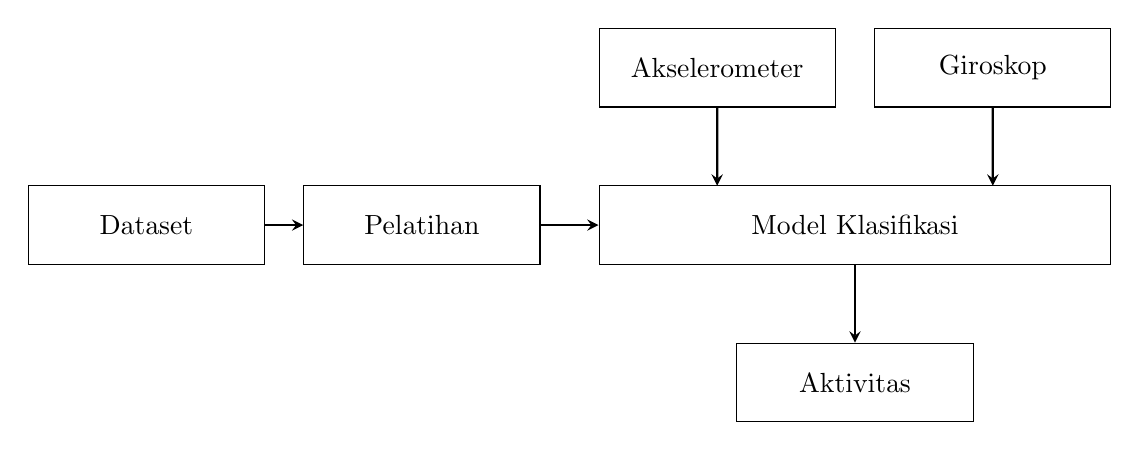
\begin{tikzpicture}[node distance=1.5cm]
        \node (dataset) [process] {Dataset};
        \node (pelatihan) [process, right of=dataset, xshift=2cm] {Pelatihan};
        \node (model-klasifikasi) [process, right of=pelatihan, xshift=4cm, minimum width=6.5cm] {Model Klasifikasi};
        \node (akselerometer) [process, above of=model-klasifikasi, xshift=-1.75cm, yshift=0.5cm] {Akselerometer};
        \node (giroskop) [process, right of=akselerometer, xshift=2cm] {Giroskop};
        % \draw (5.5,1) -- (12.5,1) -- (12.5,3.5) -- node[anchor=north] {Ponsel Cerdas} (5.5,3.5) -- (5.5,1);
        \node (aktivitas) [process, below of=model-klasifikasi, yshift=-0.5cm] {Aktivitas};

        \draw [arrow] (dataset) -- (pelatihan);
        \draw [arrow] (pelatihan) -- (model-klasifikasi);
        \draw [arrow] (akselerometer) -- (7.25,0.5);
        \draw [arrow] (giroskop) -- (10.75,0.5);
        \draw [arrow] (model-klasifikasi) -- (aktivitas);
    \end{tikzpicture}
    \caption{Diagram blok sistem}
    \label{gambar:diagram-blok-sistem}
\end{figure}

\textbf{Penjelasan diagram blok \dots}


%------------------------------------------------------------------------------
% Peralatan
%------------------------------------------------------------------------------
\section{Peralatan}
Peralatan yang digunakan untuk mendukung penelitian ini terdiri dari perangkat keras dan perangkat lunak berikut:

\subsection{Perangkat Keras}
\begin{enumerate}
    \item Laptop HP 14--015tx dengan CPU Intel Core i5--6200U 2.3 GHz dan RAM 12GB
    \item Ponsel cerdas Android dengan sensor akselerometer dan giroskop tertanam
\end{enumerate}

\subsection{Sistem Perangkat Lunak}
\begin{enumerate}
    \item Ubuntu 16.04 64 bit sebagai sistem operasi laptop
    \item TensorFlow sebagai pustaka komputasi numerik
    \item Visual Studio Code sebagai \textit{text editor} untuk menulis program sistem klasifikasi
    \item Android Studio sebagai \textit{Integrated Development Environment} (IDE) untuk mengembangkan aplikasi Android
    \item Git sebagai aplikasi pengontrol versi terdistribusi
\end{enumerate}

%------------------------------------------------------------------------------
% Rancangan Perangkat Lunak
%
% TODO:
% - Offline:
%   - Model klasifikasi
%   - Pelatihan
%   - Test
% - Online:
%   - Klasifikasi
%
%------------------------------------------------------------------------------
\section{Rancangan Perangkat Lunak}
Sistem dirancang untuk mengklasifikasikan aktivitas manusia berdasarkan data dari sensor akselerometer dan giroskop pada ponsel cerdas. Aliran data sensor pada proses klasifikasi ditunjukkan pada Gambar~\ref{gambar:aliran-data-klasifikasi}.

\begin{figure}[h!]
    \centering
    \begin{tikzpicture}[node distance=1.9cm]
        \node (masukan) [state] {Masukan};
        \node (cnn1) [state, above of=masukan, yshift=0.2cm] {Konvolusi};
        \node (cnn2) [state, above of=cnn1, yshift=0.2cm] {Konvolusi};
        \node (lstm1) [state, above of=cnn2, yshift=0.1cm] {LSTM};
        \node (lstm2) [state, above of=lstm1] {LSTM};
        \node (softmax) [state, above of=lstm2] {Softmax};
        \node (keluaran) [state, above of=softmax] {Keluaran};
        \node (loss) [state, right of=softmax, xshift=3cm] {Loss};
        \node (akurasi) [state, above of=loss] {Akurasi};
        \node (target) [state, right of=loss, yshift=1cm] {Target};
        \node (optimizer) [state, right of=lstm1, xshift=3cm] {Optimizer};

        \draw [arrow] (masukan) -- (cnn1);
        \draw [arrow] (cnn1) -- (cnn2);
        \draw [arrow] (cnn2) -- (lstm1);
        \draw [arrow] (lstm1) -- (lstm2);
        \draw [arrow] (lstm2) -- (softmax);
        \draw [arrow] (softmax) -- (keluaran);
        \draw [arrow] (keluaran) -- (loss);
        \draw [arrow] (keluaran) -- (akurasi);
        \draw [arrow] (target) -- (loss);
        \draw [arrow] (target) -- (akurasi);
        \draw [arrow] (loss) -- (optimizer);
        \draw [arrow] (optimizer) -- (cnn1);
        \draw [arrow] (optimizer) -- (cnn2);
        \draw [arrow] (optimizer) -- (lstm1);
        \draw [arrow] (optimizer) -- (lstm2);
        \draw [arrow] (optimizer) -- (softmax);
    \end{tikzpicture}
    \caption{Aliran data pada proses klasifikasi}
    \label{gambar:aliran-data-klasifikasi}
\end{figure}

\section{Model Klasifikasi}

\subsection{Data Masukan}
Data masukan adalah rangkaian data \textit{time series} dari sensor akselerometer dan giroskop. Rangkaian data tersebut diambil dari ponsel cerdas dan dikelompokkan dengan \textit{sliding window}.

Sensor akselerometer dan giroskop menghasilkan nilai bacaan dengan tiga sumbu, yaitu sumbu $x$, $y$ dan $z$. Nilai sensor akselerometer $\pmb{a}$ dan giroskop $\pmb{g}$ dinotasikan sebagai vektor~\ref{eq:vektor-akselerometer} dan~\ref{eq:vektor-giroskop}.

\begin{equation}
    \label{eq:vektor-akselerometer}
    \pmb{a} = 
    \begin{bmatrix}
        a_x \\
        a_y \\
        a_z
    \end{bmatrix}
\end{equation}

\begin{equation}
    \label{eq:vektor-giroskop}
    \pmb{g} = 
    \begin{bmatrix}
        g_x \\
        g_y \\
        g_z
    \end{bmatrix}
\end{equation}

Nilai sensor pada sumbu $x$, $y$ dan $z$ dipengaruhi oleh posisi dan arah gerak sensor. Mengingat posisi ponsel cerdas saat digunakan tidak menentu, maka perlu dicari nilai yang tidak dipengaruhi oleh arah gerak sensor, yaitu besar dari masing-masing vektor $\pmb{a}$ dan $\pmb{g}$. Besar vektor akseleromter dan giroskop dapat dicari dengan Persamaan~\ref{eq:norm-akselerometer} dan~\ref{eq:norm-giroskop}.

\begin{equation}
    \label{eq:norm-akselerometer}
    |\pmb{a}| = \sqrt{a_x^2 + a_y^2 + a_z^2}
\end{equation}

\begin{equation}
    \label{eq:norm-giroskop}
    |\pmb{g}| = \sqrt{g_x^2 + g_y^2 + g_z^2}
\end{equation}

Nilai vektor sensor dan besarnya disusun menjadi matriks akselerometer $\pmb{A}$ dan matriks giroskop $\pmb{G}$ seperti pada Persamaan~\ref{eq:matriks-akselerometer} dan~\ref{eq:matriks-giroskop}.

\begin{equation}
    \label{eq:matriks-akselerometer}
    \pmb{A} = 
    \begin{bmatrix}
        a_x & a_y & a_z & |\pmb{a}|
    \end{bmatrix}
\end{equation}

\begin{equation}
    \label{eq:matriks-giroskop}
    \pmb{G} = 
    \begin{bmatrix}
        g_x & g_y & g_z & |\pmb{g}|
    \end{bmatrix}
\end{equation}

Model klasifikasi menerima masukan tensor $\tensorsym{X}$. Jika $m_X$ jumlah baris $\tensorsym{X}$, $n_X$ jumlah kolom $\tensorsym{X}$ dan $c_X$ jumlah anggota masing-masing matriks anggota $\tensorsym{X}$, ukuran tensor $\tensorsym{X}$ adalah $m_X \times n_X \times c_X = 100 \times 2 \times 4$. Setiap baris pada tensor tersebut merupakan \textit{sample} dari matriks akselerometer $\pmb{A}$ dan giroskop $\pmb{G}$ yang diurutkan dari waktu $t_{0}$ sampai $t_{99}$.

\begin{equation}
    \label{eq:tensor-masukan}
    \tensorsym{X}_{m_X \times n_X \times c_X} =
    \begin{bmatrix}
        \pmb{A}_{t_0} & \pmb{G}_{t_0} \\
        \pmb{A}_{t_1} & \pmb{G}_{t_1} \\
        \cdots & \cdots \\
        \pmb{A}_{t_{99}} & \pmb{G}_{t_{99}} \\
    \end{bmatrix}
\end{equation}

\subsection{Lapisan Konvolusi}
Tensor $\tensorsym{X}$ dilewatkan melalui dua lapisan kovolusi untuk mencari fitur-fitur abstrak dari data sensor. Lapisan konvolusi menggunakan kernel $\tensorsym{K}$ yang merupakan tensor dengan ukuran $m_K \times n_K \times c_X \times c_K$. Nilai masing-masing anggota $\tensorsym{K}$ adalah bobot yang digunakan bersama oleh setiap jendela komputasi. Karena digunakan bersama, jumlah bobot dapat diminalisir menjadi $m_K \times n_K \times c_X$.

Setiap lapisan konvolusi juga dilengkapi oleh bias $\pmb{b}$ dan fungsi aktivasi. Fungsi aktivasi yang digunakan adalah ReLU \textit{(Rectified Linear Unit)}, didefinisikan dalam Persamaan~\ref{eq:relu}.

\begin{equation}
    g(z) = \max(0,z)
    \label{eq:relu}
\end{equation}

Nilai keluaran lapisan konvolusi dapat dihitung dengan melakukan konvolusi antara jendela komputasi $\tensorsym{I}$ dengan bobot $\tensorsym{W}$. Hasil konvolusi ditambahkan dengan bias dan dimasukkan ke dalam fungsi ReLU\@. Operasi tersebut didefinisikan sebagai

\begin{equation}
    H(i,j,k) = g((\tensorsym{I} * \tensorsym{W})(i,j,k) + \pmb{b})
    \label{eq:konvolusi-kernel}
\end{equation}

\noindent
dengan

\begin{equation}
    (\tensorsym{I} * \tensorsym{W})(i,j,k) = \sum_{m}\sum_{n}\sum_{c}I(m,n,c)W(i-m, j-n, k-c)
    \label{eq:konvolusi-3d}
\end{equation}

\noindent
Nilai optimal bobot dan bias dicari melalui tahap pelatihan.

Perhitungan tersebut dilakukan untuk setiap jendela komputasi. Berikut ini tahapan perhitungan dalam lapisan konvolusi:

\begin{enumerate}
\item Jendela komputasi $\tensorsym{I}$ dibuat dari $\tensorsym{X}$ dengan ukuran $m_K \times n_K \times c_X$
\item Untuk setiap jendela, lakukan perhitungan konvolusi dengan Persamaan~\ref{eq:konvolusi-kernel}.
\item Lakukan tahap 1 dan 2 dengan langkah antar jendela sebesar $\pmb{S}$
\item Susun hasil perhitungan setiap jendela menjadi tensor $\tensorsym{H}$
\end{enumerate}

Pada lapisan konvolusi pertama, ukuran kernel yang digunakan adalah $5 \times 2 \times 4 \times 32$ dan langkah antar jendela $\pmb{S} = [\begin{matrix}2 & 2\end{matrix}]$ sehingga menghasilkan keluaran $\tensorsym{H}^1$ dengan ukuran $50 \times 2 \times 32$.

Pada lapisan konvolusi ke dua, ukuran kernel yang digunakan adalah $5 \times 2 \times 32 \times 32$ dan langkah antar jendela $\pmb{S} = [\begin{matrix}2 & 2\end{matrix}]$ sehingga menghasilkan keluaran $\tensorsym{H}^2$ dengan ukuran $25 \times 2 \times 32$.

Perbandingan \textit{hyperparameter} lapisan konvolusi pertama dan kedua dapat dilihat pada Tabel~\ref{table:hyperparameter-lapisan-konvolusi}.

\begin{table}[h!]
    \centering
    \caption{\textit{Hyperparameter} lapisan konvolusi}
    \begin{tabular}{ |p{1.5cm}|p{3cm}|p{2cm}|p{1.5cm}|p{1.7cm}|p{2cm}| }
        \hline
        \textbf{Lapisan} & \textbf{Ukuran Kernel} & \textbf{Langkah} & \textbf{Ukuran Bias} & \textbf{Jumlah Bobot} & \textbf{Ukuran Keluaran} \\

        \hline
        1 & $5 \times 2 \times 4 \times 32$ & $[\begin{matrix}2 & 2\end{matrix}]$ & $32$ & 1280 & $50 \times 2 \times 32$ \\

        \hline
        2 & $5 \times 2 \times 32 \times 32$ & $[\begin{matrix}2 & 2\end{matrix}]$ & $32$ & 10240 & $25 \times 2 \times 32$ \\

        \hline
    \end{tabular}
    \label{table:hyperparameter-lapisan-konvolusi}
\end{table}

\subsection{Lapisan LSTM}
Setelah melalui lapisan konvolusi, hasil keluarannya dilewatkan melalui dua lapisan LSTM\@. Kedua lapisan LSTM dibuat dengan 128 \textit{hidden unit}. Masing-masing lapisan memiliki bobot antar input ke hidden $\pmb{U}$, bobot antar hidden ke output $\pmb{V}$, bobot antar hidden ke hidden $\pmb{W}$, serta bias $\pmb{b}$ dan $\pmb{c}$. Jika diberikan masukan matriks $\pmb{X}_{m \times n}$, $\pmb{x}^{(t)}$ merupakan subset dari $\pmb{X}$ pada langkah waktu $t$ dari $t = 1$ sampai $t = m$. Keluaran LSTM $\pmb{h}^{(t)}$ dapat dicari dengan Persamaan~\ref{eq:output-lstm}.

Sel-sel LSTM pada lapisan pertama disusun dengan arsitektur \textit{many-to-many} seperti pada Gambar~\ref{gambar:many-to-one}. Masukan lapisan LSTM pertama diambil dari keluaran lapisan konvolusi $\tensorsym{H}^2$ yang bentuknya diubah dari $25 \times 2 \times 32$ menjadi $25 \times 64$ dengan meratakan anggota-anggota pada dimensi ke dua dan ke tiga. Dengan begitu, lapisan LSTM pertama dapat dibentangkan menjadi $25$ langkah waktu. Masing-masing langkah waktu menerima masukan vektor yang terdiri dari $64$ fitur. Karena lapisan LSTM menggunakan arsitektur \textit{many-to-many}, memiliki $25$ langkah waktu dan disusun dari $128$ \textit{hidden unit}, maka keluaran dari lapisan ini adalah matriks fitur dengan ukuran $25 \times 128$.

\begin{figure}[h!]
    \centering
    \begin{tikzpicture}[node distance=2cm]
        \node (x1) [cell] {$x^{(1)}$};
        \node (x2) [cell, right of=x1] {$x^{(2)}$};
        \node (x25) [cell, right of=x2, xshift=1cm] {$x^{(25)}$};
        \node (h1) [cell, above of=x1] {$h^{(1)}$};
        \node (h2) [cell, above of=x2] {$h^{(2)}$};
        \node (h25) [cell, above of=x25] {$h^{(25)}$};
        \node (y1) [cell, above of=h1] {$y^{(1)}$};
        \node (y2) [cell, above of=h2] {$y^{(2)}$};
        \node (y25) [cell, above of=h25] {$y^{(25)}$};

        \draw [arrow] (x1) -- (h1);
        \draw [arrow] (x2) -- (h2);
        \draw [arrow] (x25) -- (h25);
        \draw [arrow] (h1) -- (y1);
        \draw [arrow] (h2) -- (y2);
        \draw [arrow] (h25) -- (y25);
        \draw [arrow] (h1) -- (h2);
        \draw [dashed, very thick,->] (h2) -- (h25);
    \end{tikzpicture}
    \caption{Arsitektur lapisan LSTM \textit{many-to-many}}
    \label{gambar:many-to-many}
\end{figure}

Sel-sel LSTM pada lapisan kedua disusun dengan arsitektur \textit{many-to-one} seperti pada Gambar~\ref{gambar:many-to-one}. Masukan lapisan LSTM kedua diambil dari keluaran lapisan LSTM pertama. Lapisan ini dapat dibentangkan menjadi $25$ langkah waktu dan masing-masing langkah waktu menerima masukan vektor yang terdiri dari $128$ fitur. Karena arsitektur yang digunakan merupakan arsitektur \textit{many-to-one} dan disusun dari $128$ \textit{hidden unit}, maka keluaran dari lapisan LSTM kedua hanya diambil dari keluaran pada langkah waktu terakhir, yaitu $\pmb{h}^{(t)}$ pada saat $t = m$. Dengan begitu, keluaran lapisan LSTM kedua merupakan vektor yang terdiri dari $128$ fitur.

Perbandingan \textit{hyperparameter} lapisan LSTM pertama dan kedua dapat dilihat pada Tabel~\ref{table:hyperparameter-lapisan-lstm}.

\begin{figure}[h!]
    \centering
    \begin{tikzpicture}[node distance=2cm]
        \node (x1) [cell] {$x^{(1)}$};
        \node (x2) [cell, right of=x1] {$x^{(2)}$};
        \node (x25) [cell, right of=x2, xshift=1cm] {$x^{(25)}$};
        \node (h1) [cell, above of=x1] {$h^{(1)}$};
        \node (h2) [cell, above of=x2] {$h^{(2)}$};
        \node (h25) [cell, above of=x25] {$h^{(25)}$};
        \node (y) [cell, above of=h25] {$y$};

        \draw [arrow] (x1) -- (h1);
        \draw [arrow] (x2) -- (h2);
        \draw [arrow] (x25) -- (h25);
        \draw [arrow] (h25) -- (y);
        \draw [arrow] (h1) -- (h2);
        \draw [dashed, very thick,->] (h2) -- (h25);
    \end{tikzpicture}
    \caption{Arsitektur lapisan LSTM \textit{many-to-one}}
    \label{gambar:many-to-one}
\end{figure}

\begin{table}[h!]
    \centering
    \caption{\textit{Hyperparameter} lapisan LSTM}
    \begin{tabular}{ |p{1.5cm}|p{1.5cm}|p{2cm}|p{1.7cm}|p{2.5cm}|p{2cm}| }
        \hline
        \textbf{Lapisan} & \textbf{\textit{Hidden Unit}} & \textbf{Ukuran Masukan} & \textbf{Langkah Waktu} & \textbf{Arsitektur} & \textbf{Ukuran Keluaran} \\

        \hline
        1 & $128$ & $25 \times 64$ & $25$ & \textit{many-to-many} & $25 \times 128$ \\

        \hline
        2 & $128$ & $25 \times 128$ & $25$ & \textit{many-to-one} & $128$ \\

        \hline
    \end{tabular}
    \label{table:hyperparameter-lapisan-lstm}
\end{table}

\subsection{Lapisan \textit{Softmax}}
Setelah melalui lapisan LSTM, keluarannya masuk ke lapisan \textit{softmax}. Lapisan \textit{softmax} adalah jaringan padat yang menggunakan fungsi \textit{softmax} sebagai fungsi aktivasinya. Fungsi aktivasi \textit{softmax} digunakan untuk mencari distribusi probabilitas seluruh kelas aktivitas manusia.

Jaringan padat adalah jaringan dengan neuron yang seluruhnya terhubung dengan neuron pada lapisan sebelum atau sesudahnya. Jaringan padat dengan 10 neuron dibuat dengan masukan dari hasil lapisan LSTM ke dua. Jumlah neuron tersebut dipilih sesuai dengan jumlah aktivitas yang akan diklasifikasikan.

Lapisan \textit{softmax} menerima masukan vektor $\pmb{x}$ dengan $128$ fitur. Dengan bobot $\pmb{W}$ dan bias $\pmb{b}$, keluaran lapisan ini dihitung menggunakan persamaan

\begin{equation}
    \pmb{y} = softmax(\pmb{W} \pmb{x} + \pmb{b})
\end{equation}

\noindent
dan fungsi \textit{softmax} didefinisikan sebagai

\begin{equation}
    softmax(\pmb{z})_i = \frac{\exp(z_i)}{\sum_{j=1}^n \exp(z_j)}
\end{equation}

Persamaan di atas menghasilkan vektor distribusi probabilitas dari 10 kelas aktivitas. Aktivitas yang dikenali adalah aktivitas dengan probabilitas tertinggi.


\section{Pelatihan}
Proses pelatihan jaringan dilakukan untuk mencari bobot dan bias yang optimal pada seluruh neuron dalam setiap lapisan. Optimasi bobot dan bias tersebut dilakukan dengan meminimal \textit{cost function} menggunakan algoritma optimasi berbasis \textit{gradient descent}. \textit{Cost function} yang digunakan adalah \textit{cross entropy} dan algoritma \textit{gradient descent} yang digunakan adalah RMSProp \citep{Dauphin-2015}.

\subsection{Perhitungan \textit{loss} dengan Cross Entropy}


\subsection{Optimasi dengan RMSProp}

%------------------------------------------------------------------------------
% Pengumpulan Data -> Masukkan saja ke rancangan perngkat lunak
%
% TODO:
% - Sumber Data
%   - Dataset publik
%   - Pengambilan data pada ponsel cerdas
% - Preprocessing
% - Sliding window
% - Pembagian data latih, validasi dan tes
%
%------------------------------------------------------------------------------
\section{Data Pelatihan}
Model klasifikasi dilatih dengan menggunakan dataset terbuka dari beberapa sumber, yaitu \textit{Activity Recognition Dataset} \citep{shoaib-2013}, \textit{Sensor Activity Dataset} \citep{shoaib-2014}, \textit{MobiAct Dataset} \citep{vavoulas-2016} dan \textit{Human Activity Recognition Using Smartphones Data Set} \citep{anguita-2013}. Partisipan pada keempat dataset tersebut dapat dilihat pada Tabel~\ref{table:partisipan-dataset}.

\begin{table}[h!]
    \centering
    \caption{Partisipan pengambilan data}
    \begin{tabular}{ |l|l|l|l|l|l| }
        \hline
        \textbf{Dataset} & \textbf{Partisipan} & \textbf{Laki-laki} & \textbf{Perempuan} & \textbf{Rentang Usia} \\

        \hline
        \citet{shoaib-2013} & 4 & 4 & 0 & 25 --- 30 \\

        \hline
        \citet{shoaib-2014} & 10 & 10 & 0 & 25 --- 30 \\

        \hline
        \citet{vavoulas-2016} & 57 & 39 & 15 & 20 --- 47 \\

        \hline
        \citet{anguita-2013} & 30 & --- & --- & 19 --- 48 \\

        \hline
    \end{tabular}
    \label{table:partisipan-dataset}
\end{table}

Data sensor akselerometer dan giroskop dari keempat dataset tersebut diambil dengan \textit{sampling rate} 50 Hz. \textit{Sliding window} dibuat dari setiap 100 langkah waktu dengan tumpang tindih 50\%. Dengan aturan tersebut, diperoleh data pelatihan seperti pada Tabel~\ref{table:jumlah-dataset}.

\begin{table}[h!]
    \centering
    \caption{Jumlah dataset}
    \begin{tabular}{ |l|c| }
        \hline
        \textbf{Aktivitas} & \textbf{Jumlah Sample} \\

        \hline
        Berdiri & 1000 \\

        \hline
        Duduk & 1000 \\

        \hline
        Berjalan & 1000 \\

        \hline
        Berlari & 1000 \\

        \hline
        Bersepeda & 1000 \\

        \hline
        Menaiki Tangga & 1000 \\

        \hline
        Menuruni Tangga & 1000 \\

        \hline
    \end{tabular}
    \label{table:jumlah-dataset}
\end{table}

Data tersebut dibagi untuk pelatihan dan pengujian. Seluruh data terlebih dulu diacak, lalu 70\% data diambil untuk data latih dan 30\% untuk data uji. Hasil pembagian data dapat dilihat pada Tabel~\ref{table:pembagian-data-latih-uji}.

\begin{table}[h!]
    \centering
    \caption{Pembagian data latih dan data uji}
    \begin{tabular}{ |l|c| }
        \hline
        \textbf{Data} & \textbf{Jumlah Sample} \\

        \hline
        Data Latih & 1000 \\

        \hline
        Data Uji & 1000 \\

        \hline
    \end{tabular}
    \label{table:pembagian-data-latih-uji}
\end{table}


\section{Klasifikasi Pada Ponsel Cerdas}
Proses klasifikasi pada ponsel cerdas ditunjukkan pada Gambar~\ref{gambar:diagram-alir-klasifikasi-ponsel-cerdas}. Sensor akselerometer dan giroskop dibaca dengan \textit{sampling rate} 50 Hz. Masing-masing sensor menghasilkan data dengan tiga sumbu, sehingga satu kali pembacaan menghasilkan enam data. Hasil bacaannya dikumpulkan menjadi jendela berisi 100 sample dengan tumpang tindih 50\%. Dengan begitu, satu jendela data terdiri dari pembacaan sensor selama dua detik dan jendela baru dibuat setiap satu detik. Setelah jendela terpenuhi, jendela tersebut dijadikan sebagai masukan model klasifikasi yang telah dibuat. Proses ini menghasilkan kelas aktivitas manusia yang sesuai dengan bacaan sensor.

\begin{figure}[h]
    \centering
    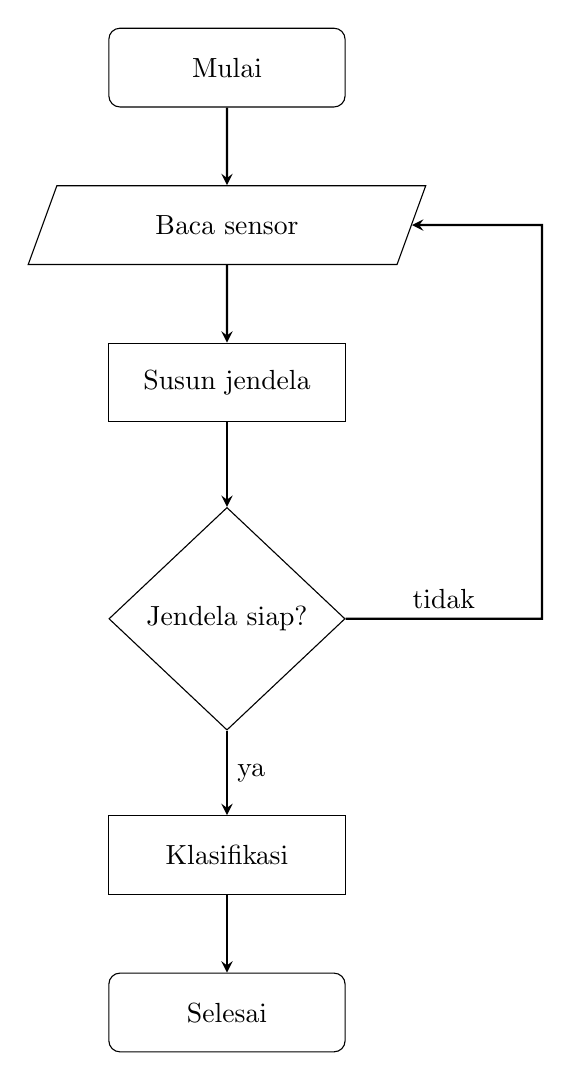
\begin{tikzpicture}[node distance=2cm]
        \node (mulai) [startstop] {Mulai};
        \node (baca-sensor) [io, below of=mulai] {Baca sensor};
        \node (susun-jendela) [process, below of=baca-sensor] {Susun jendela};
        \node (jendela-siap) [decision, below of=susun-jendela, yshift=-1cm] {Jendela siap?};
        \node (klasifikasi) [process, below of=jendela-siap, yshift=-1cm] {Klasifikasi};
        \node (selesai) [startstop, below of=klasifikasi] {Selesai};

        \draw [arrow] (mulai) -- (baca-sensor);
        \draw [arrow] (baca-sensor) -- (susun-jendela);
        \draw [arrow] (susun-jendela) -- (jendela-siap);
        \draw [arrow] (jendela-siap) -- node[anchor=south] {tidak} (4,-7) -- (4,-2) -- (baca-sensor);
        \draw [arrow] (jendela-siap) -- node[anchor=west] {ya} (klasifikasi);
        \draw [arrow] (klasifikasi) -- (selesai);
    \end{tikzpicture}
    \caption{Diagram alir klasifikasi pada ponsel cerdas}
    \label{gambar:diagram-alir-klasifikasi-ponsel-cerdas}
\end{figure}

%------------------------------------------------------------------------------
% Pengujian
%
% Tabel: indikator keberhasilan
% Menjawab judul rumusan masalah
%------------------------------------------------------------------------------
\section{Rencana Pengujian}
Pengujian dilakukan untuk mengetahui kemampuan klasifikasi dari model yang telah dibuat. Terdapat tiga parameter yang diuji, yaitu akurasi klasifikasi \textit{offline}, akurasi klasifikasi \textit{online} dan kecepatan klasifikasi pada ponsel cerdas.

Pada pengujian klasifikasi \textit{offline}, kemampuan model klasifikasi diukur berdasarkan akurasi klasifikasi pada data uji. Model klasifikasi menerima data uji yang diambil secara acak dari dataset dan terpisah dari data latih. Keluaran dari proses klasifikasi dibandingkan dengan label data tersebut.

Pada pengujian klasifikasi \textit{online}, kemampuan model klasifikasi diukur berdasarkan akurasi klasifikasi pada data sensor ponsel cerdas yang diambil dan diolah secara \textit{real time}. Pengujian dilakukan oleh ? partisipan yang terdiri dari ? laki-laki dan ? perempuan. Partisipan memilih aktivitas yang akan diuji, lalu aktivitas tersebut dibandingkan dengan hasil klasifikasi dari data sensor. Ponsel cerdas ditempatkan di saku celana dengan posisi acak. Setiap partisipan melakukan pengujian selama ? menit untuk masing-masing aktivitas.

Pengujian kecepatan klasifikasi dilakukan bersamaan dengan pengujian klasifikasi \textit{online}. Pengujian dilakukan dengan mengukur waktu yang dibutuhkan oleh setiap siklus klasifikasi, dimulai dari pengambilan data sensor sampai diperoleh kelas aktivitas dari data tersebut. Pengukuran ini dilakukan dengan beberapa model ponsel cerdas dengan kemampuan pemrosesan yang berbeda.

Ketiga pengujian ini dilakukan dengan indikator pencapaian yang ditunjukkan pada Tabel~\ref{table:rencana-pengujian}.

\begin{table}[h!]
    \centering
    \caption{Rencana Pengujian}
    \begin{tabular}{ |p{0.5cm}|p{5cm}|p{7.5cm}| }
        \hline
        \textbf{No} & \textbf{Parameter} & \textbf{Pencapaian} \\

        \hline
        1 & Pengujian akurasi klasifikasi \textit{offline} & Didapatkan tingkat akurasi \dots pada data uji  \\

        \hline
        2 & Pengujian akurasi klasifikasi \textit{online} & Didapatkan tingkat akurasi \dots pada klasifikasi secara \textit{online}\\
        
        \hline
        3 & Pengujian kecepatan klasifikasi pada ponsel cerdas & Klasifikasi dapat dilakukan secara \textit{real time} pada ponsel cerdas \\

        \hline
    \end{tabular}
    \label{table:rencana-pengujian}
\end{table}

\chapter{IMPLEMENTASI}

% \section{Implementasi Perangkat Lunak}
\section{Implementasi Model Klasifikasi}
Model klasifikasi diimplementasikan dalam bahasa Python menggunakan pustaka TensorFlow. Pustaka-pustaka yang dibutuhkan di-\mintinline{python}{import} pada Gambar~\ref{listing:har-import}.

\begin{figure}[h]
\begin{minted}[linenos=true]{python}
import tensorflow as tf
import tensorflow.contrib.slim as slim
import data
\end{minted}
\caption{\textit{Import} pustaka yang dibutuhkan model klasifikasi}
\label{listing:har-import}
\end{figure}


Model klasifikasi didefiniskan sebagai kelas \mintinline{python}{HARConvLSTM}. Gambar~\ref{listing:har-HARConvLSTM-constructor} menunjukkan \textit{constructor} dari kelas \mintinline{python}{HARConvLSTM}.

\begin{figure}[h]
    \inputminted[firstline=14,firstnumber=14,lastline=31,fontsize=\scriptsize]{python}{../har/har.py}
    \caption{\textit{Constructor} kelas HARConvLSTM}
    \label{listing:har-HARConvLSTM-constructor}
\end{figure}

Pada \textit{constructor} tersebut didefinikan beberapa atribut dari kelas \mintinline{python}{HARConvLSTM}. Atribut \mintinline{python}{self.features} adalah atribut untuk menyimpan data sensor yang akan diklasifikasi dan \mintinline{python}{self.target} adalah target aktivitas dari data tersebut. Atribut \mintinline{python}{self.features} menyimpan data sensor akselerometer dan giroskop sebagai matriks berukuran $1 \times 600$ dengan susunan

\begin{equation}
    \mintinline{python}{self.features} = [a_x^1, a_y^1, a_z^1, g_x^1, g_y^1, g_z^1,\dots, a_x^{100}, a_y^{100}, a_z^{100}, g_x^{100}, g_y^{100}, g_z^{100}]
\end{equation}

Graf komputasi dibuat sesuai dengan arsitektur yang telah disusun. Pada baris $23$ dan $24$, data masukan dikondisikan menjadi tensor \mintinline{python}{conv_input} seperti pada Persamaan~\ref{eq:tensor-masukan}. Perhitungan besar vektor data sensor dilakukan dengan metode \mintinline{python}{self.__preprocessing()}. Hasil dari metode tersebut diubah bentuknya dari $100 \times 8$ menjadi $100 \times 2 \times 4$ dengan instruksi pada baris $24$. Selanjutnya dua lapisan konvolusi didefinikan berurutan pada baris $25$ dan $26$ dengan fungsi \mintinline{python}{self.__conv_layer()}. Lapisan konvolusi pertama menerima input dari tensor \mintinline{python}{conv1_input} dan menghasilkan tensor \mintinline{python}{conv1}. Kemudian tensor \mintinline{python}{conv1} masuk ke lapisan konvolusi ke dua yang menghasilkan tensor \mintinline{python}{conv2}.

Dua lapisan LSTM dibuat dengan metode \mintinline{python}{self.__lstm_layer()} pada baris $28$. Lapisan LSTM ini menerima tensor \mintinline{python}{lstm_input} sebagai masukannya. Tensor \mintinline{python}{lstm_input} dibuat dengan mengubah bentuk tensor \mintinline{python}{conv2} dari $25 \times 2 \times 32$ menjadi $25 \times 64$ pada baris $27$. Setelah itu keluaran dari lapisan LSTM dimasukkan ke lapisan softmax pada baris $29$.

\begin{figure}[h]
    \inputminted[firstline=32,firstnumber=32,lastline=48,gobble=4]{python}{../har/har.py}
    \caption{Implementasi pengondisian data masukan}
    \label{listing:har-masukan}
\end{figure}

Metode \mintinline{python}{self.__preprocessing()} diimplementasikan pada Gambar~\ref{listing:har-masukan}. Metode ini digunakan untuk menghitung besar dari vektor akselerometer dan giroskop dan membentuk matriks akselerometer dan giroskop seperti pada Persamaan~\ref{eq:matriks-akselerometer} dan~\ref{eq:matriks-giroskop}. Besar vektor akselerometer dan giroskop dihitung dengan memanggi metode \mintinline{python}{self.__magnitude()} pada baris $38$ dan $39$. Adapun metode \mintinline{python}{self.__magnitude()} didefinisikan pada baris $43 - 48$.

Pembuatan lapisan konvolusi dengan metode \mintinline{python}{self.__conv_layer()} diimplementasikan pada Gambar~\ref{listing:har-konvolusi}. Metode tersebut menerima parameter \mintinline{python}{tensor_in} sebagai masukan lapisan konvolusi dan \mintinline{python}{filters} sebagai ukuran kernel yang digunakan. Bobot dan bias jaringan saraf diinisialisasi pada baris $52 - 53$ dengan metode \mintinline{python}{self.__weight_variable()} dan \mintinline{python}{self.__bias_variable()}. Kedua metode tersebut menginisialisasi nilai-nilai secara acak dari distribusi normal, seperti yang diimplementasikan pada baris $59 - 65$ dan $67 - 73$. Selanjutnya pada baris $55 - 57$ konvolusi dilakukan terhadap masukan dan bobot sesuai dengan Persamaan~\ref{eq:konvolusi-3d}, lalu hasilnya ditambahkan dengan bias dan dimasukkan pada fungsi aktivasi ReLU seperti pada Persamaan~\ref{eq:konvolusi-kernel}.

\begin{figure}[h]
    \inputminted[firstline=50,firstnumber=50,lastline=73,gobble=4]{python}{../har/har.py}
    \caption{Implementasi lapisan konvolusi}
    \label{listing:har-konvolusi}
\end{figure}

Gambar~\ref{listing:har-lstm} mengimplementasikan metode \mintinline{python}{self.__lstm_layer()} untuk pembuatan lapisan LSTM\@. Metode tersebut menerima parameter \mintinline{python}{tensor_in} sebagai masukan lapisan LSTM, \mintinline{python}{num_unit} sebagai jumlah sel LSTM pada masing-masing lapisan dan \mintinline{python}{num_layers} sebagai jumlah lapisan LSTM yang akan dibuat. Sesuai dengan paramter yang diberikan, sejumlah \mintinline{python}{num_layers} lapisan LSTM akan dibuat dengan \mintinline{python}{num_units} sel LSTM pada masing-masing lapisannya. Lapisan LSTM pertama menerima masukan dari \mintinline{python}{tensor_in}, sedangkan lapisan selanjutnya menerima masukan dari keluaran lapisan sebelumnya. Sesuai dengan arsitektur \textit{many-to-one}, pada baris $86$ dikembalikan keluaran pada langkah waktu terakhir dari lapisan LSTM terakhir.

\begin{figure}[h]
    \inputminted[firstline=75,firstnumber=75,lastline=86,gobble=4]{python}{../har/har.py}
    \caption{Implementasi lapisan LSTM}
    \label{listing:har-lstm}
\end{figure}

% \section{Implementasi Pelatihan}

% \begin{figure}[h]
%     \inputminted[firstline=89,firstnumber=89,lastline=104,gobble=4]{python}{../har/har.py}
%     \caption{Implementasi \textit{cross entropy} dan RMSProp}
%     \label{listing:har-cross-entropy-rmsprop}
% \end{figure}

% \begin{figure}[h]
%     \inputminted[firstline=147,firstnumber=147,lastline=176,gobble=4]{python}{../har/har.py}
%     \caption{Implementasi proses pelatihan}
%     \label{listing:har-pelatihan}
% \end{figure}

% \begin{figure}[h]
%     \inputminted[firstline=178,firstnumber=178,lastline=190,gobble=4]{python}{../har/har.py}
%     \caption{Implementasi pengujian model}
%     \label{listing:har-pengujian-model}
% \end{figure}


\section{Implementasi Pengambilan dan Pengondisian Data}
Data latih dan data uji dipersiapkan dengan fungsi \mintinline{python}{get()} yang diimplementasikan pada Gambar~\ref{listing:data-pengambilan-data-latih-uji}. Fungsi tersebut menerima parameter \mintinline{python}{filenames} sebagai daftar nama file dataset, \mintinline{python}{num_target} sebagai jumlah kelas aktivitas yang akan dikenali, \mintinline{python}{windows_size} sebagai lebar jendela, \mintinline{python}{overlap} sebagai aturan tumpang tindih jendela dan \mintinline{python}{divider} sebagai pembagi data latih dan uji.

\begin{figure}[h]
    \inputminted[firstline=5,firstnumber=5,lastline=22]{python}{../har/data.py}
    \caption{Implementasi pengambilan data latih dan data uji}
    \label{listing:data-pengambilan-data-latih-uji}
\end{figure}

Pada baris ke $6$, fungsi \mintinline{python}{load()} mengekstrak data sensor dan target aktivitas dari file serta mengaplikasikan \textit{sliding window} pada data tersebut. Lalu hasil \textit{sliding window} diacak dengan fungsi \mintinline{python}{shuffle()} pada baris $7$. Jika diberikan parameter \mintinline{python}{divider}, maka data dan target dibagi untuk data latih dan data uji dengan fungsi \mintinline{python}{divide()} pada baris $10 - 11$.

\begin{figure}[h]
    \inputminted[firstline=25,firstnumber=25,lastline=44]{python}{../har/data.py}
    \caption{Implementasi pengambilan data dari file}
    \label{listing:data-pengambilan-data-file}
\end{figure}

Implementasi fungsi \mintinline{python}{load()} dapat dilihat pada Gambar~\ref{listing:data-pengambilan-data-file}. Pada baris $30$ data dari seluruh \mintinline{python}{filename} diekstrak menghasilkan tuple \mintinline{python}{file} dengan anggota \mintinline{python}{data} dan \mintinline{python}{target}. Baris $36$ mengaplikasikan fungsi \textit{sliding\_window}, lalu data dan target dari seluruh \mintinline{python}{filename} digabungkan pada baris $37-42$.

Proses \textit{sliding window} diimplementasikan pada Gambar~\ref{listing:data-sliding-window}. Pada baris $51-56$ dilakukan iterasi pada seluruh \mintinline{python}{data} dan \mintinline{python}{target} untuk membuat jendela dengan ukuran \mintinline{python}{windows_size} dan dan aturan tumpang tindih \mintinline{python}{overlap}.

\begin{figure}[h]
    \inputminted[firstline=47,firstnumber=47,lastline=58]{python}{../har/data.py}
    \caption{Implementasi \textit{sliding windows}}
    \label{listing:data-sliding-window}
\end{figure}

Setelah diperoleh rangkaian jendela \mintinline{python}{data} dan \mintinline{python}{target} dari fungsi \mintinline{python}{load()}, rangkaian jendela tersebut diacak fungsi \mintinline{python}{shuffle()} yang diimplementasikan pada Gambar~\ref{listing:data-pengacakan-data}. Pada baris $62-63$, \mintinline{python}{data} dan \mintinline{python}{target} digabungkan agar urutan pasangan keduanya tetap konsisten setelah melalui proses pengacakan. Pengacakan dilakukan pada baris $64$, lalu \mintinline{python}{data} dan \mintinline{python}{target} dipisahkan kembali pada baris $66-67$.

\begin{figure}[h]
    \inputminted[firstline=61,firstnumber=61,lastline=69]{python}{../har/data.py}
    \caption{Implementasi pengacakan data}
    \label{listing:data-pengacakan-data}
\end{figure}

Pembagian data latih dan data uji dilakukan dengan fungsi \mintinline{python}{divide()} yang diimplementasikan pada Gambar~\ref{listing:data-pembagian-data-latih-uji}. Fungsi \mintinline{python}{divide()} menerima parameter \mintinline{python}{arr} sebagai data yang akan dibagi dan \mintinline{python}{divider} sebagai rasio pembagian data. Sejumlah $(divider \times 100) \%$ data dari \mintinline{python}{arr} dijadikan data latih dan sisanya dijadikan data uji.

\begin{figure}[h]
    \inputminted[firstline=72,firstnumber=72,lastline=76]{python}{../har/data.py}
    \caption{Implementasi pembagian data latih dan data uji}
    \label{listing:data-pembagian-data-latih-uji}
\end{figure}

\section{Implementasi Klasifikasi Pada Ponsel Cerdas}
Sistem diimplemantasikan pada ponsel cerdas dengan sistem operasi Android. Proses klasifikasi dimulai dengan pengambilan dan pengondisian data sensor akselerometer dan giroskop. Kedua sensor tersebut diinisialisasi oleh kelas \mintinline{java}{SensorReader} pada Gambar~\ref{listing:inisialisasi-sensor}. \textit{Constructor} \mintinline{java}{SensorReader()} menerima \mintinline{java}{List} berisi jenis sensor yang akan dibaca, lalu pada baris $28-30$ seluruhnya didaftarkan untuk pembacaan dengan fungsi \mintinline{java}{registerSensorIfAvailable()}.

\begin{figure}[h]
    \inputminted[firstline=14,firstnumber=14,lastline=32]{java}{../aktvtas/app/src/main/java/org/elins/aktvtas/sensor/SensorReader.java}
    \caption{Inisialisasi sensor}
    \label{listing:inisialisasi-sensor}
\end{figure}

Fungsi \mintinline{java}{registerSensorIfAvailable()} pada Gambar~\ref{listing:mendaftarkan-sensor} digunakan untuk mendaftarkan \textit{listener} pada masing-masing sensor dan mengatur \textit{sampling rate} menjadi 50 Hz. Sehingga setiap 20 milisekon, ketika bacaan baru dari sensor telah siap, fungsi \textit{callback} \mintinline{java}{onSensorDataReady()} akan dipanggil.

\begin{figure}[h]
    \inputminted[firstline=38,firstnumber=38,lastline=44,gobble=4]{java}{../aktvtas/app/src/main/java/org/elins/aktvtas/sensor/SensorReader.java}
    \caption{Mendaftarkan sensor}
    \label{listing:mendaftarkan-sensor}
\end{figure}

Data sensor disimpan dan dikelola dalam dua struktur data, yaitu \mintinline{java}{SensorData} dan \mintinline{java}{SensorDataSequence}. Struktur \mintinline{java}{SensorData} (Gambar~\ref{listing:sensor-data}) digunakan untuk menyimpan dan mengelola data satu sensor dalam satu waktu, sedangkan struktur \mintinline{java}{SensorDataSequence} (Gambar~\ref{listing:sensor-data-sequence}) digunakan untuk menyimpan dan mengelola jendela data dari seluruh sensor.

\begin{figure}[h]
    \inputminted[firstline=6,firstnumber=6,lastline=16]{java}{../aktvtas/app/src/main/java/org/elins/aktvtas/sensor/SensorData.java}
    \caption{Struktur SensorData}
    \label{listing:sensor-data}
\end{figure}

\begin{figure}[h]
    \inputminted[firstline=9,firstnumber=9,lastline=13]{java}{../aktvtas/app/src/main/java/org/elins/aktvtas/sensor/SensorDataSequence.java}
    \caption{Struktur SensorDataSequence}
    \label{listing:sensor-data-sequence}
\end{figure}

Pengambilan data sensor dilakukan dalam kelas \mintinline{java}{SensorService}. Kelas \mintinline{java}{SensorService} mengimplementasikan \textit{interface} \mintinline{java}{SensorReaderEvent} dari kelas \mintinline{java}{SensorReader}, sehingga setiap kali bacaan sensor baru tersedia, implementasi metode \mintinline{java}{onSensorDataReady()} pada kelas \mintinline{java}{SensorService} akan dipanggil (Gambar~\ref{listing:callback-sensor-ready}). Pada baris $47$, data sensor dibaca dan menghasilkan \mintinline{java}{List} berisi \mintinline{java}{SensorData} terbaru dari seluruh sensor. Kemudian data tersebut disusun menjadi \mintinline{java}{SensorDataSequence} pada baris $59-52$.

\begin{figure}[h]
    \inputminted[firstline=45,firstnumber=45,lastline=56,gobble=4]{java}{../aktvtas/app/src/main/java/org/elins/aktvtas/sensor/SensorService.java}
    \caption{Struktur SensorDataSequence}
    \label{listing:callback-sensor-ready}
\end{figure}

Pengenalan aktivitas manusia dilakukan secara \textit{real time} pada ponsel cerdas dengan kelas \mintinline{java}{PredictionService} yang memperluas kelas \mintinline{java}{SensorService}. Kelas \mintinline{java}{PredictionService} mengimplementasikan metode \mintinline{java}{onSensorDataReady()} seperti pada Gambar~\ref{listing:callback-sensor-ready-prediction}.

\begin{figure}[h]
    \inputminted[firstline=97,firstnumber=97,lastline=123,gobble=4]{java}{../aktvtas/app/src/main/java/org/elins/aktvtas/PredictionService.java}
    \caption{Struktur SensorDataSequence}
    \label{listing:callback-sensor-ready-prediction}
\end{figure}

Pada baris $99$, metode \mintinline{java}{super.onSensorDataReady()} dipanggil untuk menjalankan implementasi \mintinline{java}{onSensorDataReady()} pada kelas \mintinline{java}{SensorService}. Pemanggilan metode tersebut dilakukan untuk menyusun bacaan sensor menjadi struktur \mintinline{java}{SensorDataSequence}. Saat ukuran \mintinline{java}{SensorDataSequence} telah sesuai dengan ukuran jendela yang diinginkan, aktivitas diklasifikasikan dengan memanggil metode \mintinline{java}{classifier.classify(SensorDataSequence)} pada baris $104$.

Akurasi pengenalan dihitung pada baris $116-123$. Pengenalan yang tepat diketahui dengan membandingkan hasil klasifikasi dengan referensi. Pada baris $122$, tingkat akurasi pengenalan dihitung dengan persamaan

\begin{equation}
    accuracy = \frac{correctPrediction}{totalPrediction} \times 100
\end{equation}

Klasifikasi dengan metode \mintinline{java}{classify()} diimplementasikan pada Gambar~\ref{listing:klasifikasi-aktivitas}. Metode tersebut menerima parameter \mintinline{java}{SensorDataSequence} sebagai masukan dari model klasifikasi. Pada baris $35$, \mintinline{java}{SensorDataSequence} diratakan menjadi matriks satu dimensi dengan memanggil metode \mintinline{java}{sequence.flatten()}. Pada baris $44-46$, data dimasukkan ke model klasifikasi dengan \mintinline{java}{inferenceInterface.feed()}, klasifikasi dijalankan dengan \mintinline{java}{inferenceInterface.run()} dan keluaran diambil dengan \mintinline{java}{inferenceInterface.fetch()}. Objek \mintinline{java}{inferenceInterface} sendiri merupakan \textit{instance} dari kelas \mintinline{java}{TensorFlowInferenceInterface}. Hasil klasifikasi terbaik dicari dengan metode \mintinline{java}{findBestClassification()}.

\begin{figure}[h]
    \inputminted[firstline=34,firstnumber=34,lastline=56,gobble=4]{java}{../aktvtas/app/src/main/java/org/elins/aktvtas/human/HumanActivityClassifier.java}
    \caption{Pengklasifikasian Aktivitas Manusia}
    \label{listing:klasifikasi-aktivitas}
\end{figure}

\section{Implementasi Pengujian}

\chapter{HASIL DAN PEMBAHASAN}

\section{Pengujian Hyperparameter}

Pengujian \textit{hyperparameter} dilakukan untuk mencari model klasifikasi terbaik, yaitu model yang memenuhi beberapa kriteria berikut:

\begin{enumerate}
    \item Model dapat melakukan klasifikasi dengan baik, ditunjukkan dengan tingkat akurasi klasifikasi yang tinggi terhadap data uji.
    \item Model dapat menyamaratakan dengan baik, ditunjukkan dengan perbedaan yang tidak signifikan antara akurasi klasifikasi data latih dengan akurasi data validasi dan data uji.
    \item Kompleksitas model minimal, sehingga mengurangi beban komputasi dan klasifikasi dapat dilakukan secara \textit{realtime} pada ponsel cerdas.
\end{enumerate}

Variasi \textit{hyperparameter} ditunjukkan pada Tabel~\ref{table:variasi-hyperparameter}. Pengujian dilakukan sebanyak 31 kali dengan variasi \textit{hyperparameter} yang dipilih secara acak. Masing-masing variasi dilatih dalam maksimal 30 \textit{epoch}.

\begin{table}[h!]
    \centering
    \caption{Variasi hyperparameter}
    \begin{tabular}{ |l|c| }
        \hline
        Hyperparameter & Variasi \\

        \hline
        Jumlah lapisan konvolusi & $2 - 4$ \\

        \hline
        Jumlah output konvolusi & $32, 64, 128$ \\

        \hline
        Jumlah lapisan LSTM & $2 - 4$ \\

        \hline
        Jumlah unit LSTM & $32, 64, 128$ \\

        \hline
        Peluang \textit{dropout} & $0,2 - 0,8$ \\

        \hline
        Laju pembelajaran ($\alpha$) & $10^{-4} - 10^{-3}$ \\

        \hline
    \end{tabular}
    \label{table:variasi-hyperparameter}
\end{table}

Hasil pengujian dapat dilihat pada Tabel~\ref{table:hasil-pengujian-hyperparameter}. Perbedaan \textit{hyperparameter} yang digunakan menghasilkan tingkat akurasi klasifikasi yang berbeda. Berdasarkan hasil tersebut, diambil tiga \textit{hyperparameter} dengan akurasi terbaik untuk dibandingkan lebih lanjut, yaitu \textit{hyperparameter} pada variasi nomor 8, 17 dan 28.

\begin{table}[h!]
    \centering
    \caption{Hasil pengujian \textit{hyperparameter}}
    \pgfplotstabletypeset[
        col sep=comma,
        before row=\hline,every last row/.style={after row=\hline},
        display columns/0/.style={column type=|c|},
        display columns/1/.style={string type, column type=l|},
        display columns/2/.style={string type, column type=l|},
        display columns/3/.style={column type=c|},
        display columns/4/.style={column type=c|,column name=$\alpha$},
        display columns/5/.style={column type=c|,precision=5},
    ]{data/pelatihan/hyperparameter.csv}
    \label{table:hasil-pengujian-hyperparameter}
\end{table}

Variasi 8 menggunakan empat lapisan konvolusi dan empat lapisan LSTM\@. Keempat lapisan konvolusi menggunakan kernel dengan $64$ output. Lapisan konvolusi pertama menerima input tensor dengan dimensi $100 \times 8$ dan lapisan konvolusi terakhir menghasilkan output tensor dengan ukuran $100 \times 64$. Keempat lapisan LSTM memiliki $32$ unit LSTM\@. Lapisan LSTM pertama menerima input tensor dari output konvolusi dan lapisan LSTM terakhir menghasilkan output tensor dengan ukuran $1 \times 32$. Variasi ini dilatih dengan peluang \textit{dropout} $0.79$ dan laju pembelajaran $1.46 \times 10^{-4}$.

Proses pelatihan variasi 8 dapat dilihat pada Gambar~\ref{gambar:run8-training}. Grafik tersebut menunjukkan peningkatan akurasi klasifikasi dalam proses pelatihan terhadap data latih dan data validasi. Model akhir diambil dari kondisi jaringan saat menghasilkan akurasi terbaik terhadap data validasi, yaitu pada iterasi ke $5069$ dengan akurasi $0.912331$. Pada iterasi yang sama, akurasi terhadap data latih adalah $0.982142$ dan akurasi terhadap data uji adalah $0.91169$.

\begin{figure}[h!]
    \centering
    \includegraphics[width=14cm]{data/pelatihan/run8-accuracy.png}
    \caption{Proses pelatihan pada variasi 8}.
    \label{gambar:run8-training}
\end{figure}

\textit{Confusion matrix} variasi 8 dapat dilihat pada Gambar~\ref{gambar:run8-confusion-martix}. Pada gambar tersebut dapat dilihat bahwa klasifikasi dilakukan dengan baik pada aktivitas berdiri (96,9\%), duduk (94,9\%) dan lari (96,9\%). Aktivitas jalan memiliki akurasi 87,6\% dan \textit{false negative} yang cukup besar pada naik tangga (8,5\%) dan turun tangga (3,9\%). Aktivitas naik dan turun tangga memiliki klasifikasi terburuk dengan akurasi masing-masing 78,6\% dan 78,4\%, dengan \textit{false negative} tersebar pada seluruh aktivitas lainnya.

\begin{figure}[h!]
    \centering
    \includegraphics[width=13cm]{gambar/hasil-pembahasan/run8-confusion-matrix.png}
    \caption{\textit{Confusion matrix} pada variasi 8}.
    \label{gambar:run8-confusion-martix}
\end{figure}

Variasi 17 menggunakan tiga lapisan konvolusi dan tiga lapisan LSTM\@. Masing-masing lapisan konvolusi menggunakan kernel dengan $64$ output. Lapisan konvolusi pertama menerima input tensor dengan dimensi $100 \times 8$ dan lapisan konvolusi terakhir menghasilkan output tensor dengan ukuran $100 \times 64$. Masing-masing lapisan LSTM memiliki $64$ unit LSTM\@. Lapisan LSTM pertama menerima input tensor dari output konvolusi dan lapisan LSTM terakhir menghasilkan output tensor dengan ukuran $1 \times 64$. Variasi ini dilatih dengan peluang \textit{dropout} $0.59$ dan laju pembelajaran $2.81 \times 10^{-4}$.

Proses pelatihan variasi 17 dapat dilihat pada Gambar~\ref{gambar:run17-training}. Model akhir diambil dari kondisi jaringan saat menghasilkan akurasi terbaik terhadap data validasi, yaitu pada iterasi ke $4394$ dengan akurasi $0.929793$. Pada iterasi yang sama, akurasi terhadap data latih adalah $1.0$ dan akurasi terhadap data uji  $0.93652$.

\begin{figure}[h!]
    \centering
    \includegraphics[width=14cm]{data/pelatihan/run17-accuracy.png}
    \caption{Proses pelatihan pada variasi 17}.
    \label{gambar:run17-training}
\end{figure}

\textit{Confusion matrix} variasi 17 dapat dilihat pada Gambar~\ref{gambar:run17-confusion-martix}. Pada gambar tersebut dapat dilihat bahwa klasifikasi dilakukan dengan baik pada aktivitas berdiri (97,2\%), duduk (93,4\%) dan jalan (96,1\%). Aktivitas lari memiliki akurasi 85,5\% dan \textit{false negative} yang cukup besar pada jalan (8,6\%) dan turun tangga (5,7\%). Aktivitas naik dan turun tangga memiliki akurasi masing-masing 81,2\% dan 82,4\%, dengan \textit{false negative} tersebar pada seluruh aktivitas lainnya.

\begin{figure}[h!]
    \centering
    \includegraphics[width=13cm]{gambar/hasil-pembahasan/run17-confusion-matrix.png}
    \caption{\textit{Confusion matrix} pada variasi 17}.
    \label{gambar:run17-confusion-martix}
\end{figure}

Variasi 28 menggunakan empat lapisan konvolusi dan tiga lapisan LSTM\@. Masing-masing lapisan konvolusi menggunakan kernel dengan $64$ output. Lapisan konvolusi pertama menerima input tensor dengan dimensi $100 \times 8$ dan lapisan konvolusi terakhir menghasilkan output tensor dengan ukuran $100 \times 64$. Masing-masing lapisan LSTM memiliki $32$ unit LSTM\@. Lapisan LSTM pertama menerima input tensor dari output konvolusi dan lapisan LSTM terakhir menghasilkan output tensor dengan ukuran $1 \times 32$. Variasi ini dilatih dengan peluang \textit{dropout} $0.76$ dan laju pembelajaran $4.14 \times 10^{-4}$.

Proses pelatihan variasi 28 dapat dilihat pada Gambar~\ref{gambar:run34-training}. Model akhir diambil dari kondisi jaringan saat menghasilkan akurasi terbaik terhadap data validasi, yaitu pada iterasi ke $4901$ dengan akurasi $0.896472$. Pada iterasi yang sama, akurasi terhadap data latih adalah $0.9375$ dan akurasi terhadap data uji  $0.93153$.

\begin{figure}[h!]
    \centering
    \includegraphics[width=14cm]{data/pelatihan/run34-accuracy.png}
    \caption{Proses pelatihan pada variasi 28}.
    \label{gambar:run34-training}
\end{figure}

\textit{Confusion matrix} variasi 28 dapat dilihat pada Gambar~\ref{gambar:run34-confusion-martix}. Pada gambar tersebut dapat dilihat bahwa klasifikasi dilakukan dengan baik pada aktivitas berdiri (99,4\%), jalan (98,4\%) dan lari (94,6\%). Aktivitas duduk memiliki akurasi 77,4\% dan \textit{false negative} yang besar pada jalan (16,6\%). Aktivitas naik dan turun tangga memiliki akurasi masing-masing 62,2\% dan 58,3\%, dengan \textit{false negative} tersebar pada seluruh aktivitas lainnya.

\begin{figure}[h!]
    \centering
    \includegraphics[width=13cm]{gambar/hasil-pembahasan/run34-confusion-matrix.png}
    \caption{\textit{Confusion matrix} pada variasi 28}.
    \label{gambar:run34-confusion-martix}
\end{figure}

Hasil pengujian variasi 8, 17 dan 28 dibandingkan dalam Tabel~\ref{table:perbandingan-model-klasifikasi}. Ketiga variasi tersebut memiliki kelebihan dan kekurangannya masing-masing. Variasi nomor 8 memperoleh akurasi tertinggi pada aktivitas duduk dan lari, namun memperoleh akurasi terendah pada aktivitas berdiri, jalan dan rata-rata akurasi. Variasi nomor 17 memperoleh akurasi tertinggi pada aktivitas naik tangga, turun tangga dan rata-rata akurasi, namun memperoleh akurasi terendah pada aktivitas duduk dan lari. Selain itu variasi nomor 17 juga memiliki arsitektur yang paling sederhana diantara variasi lainnya. Variasi nomor 28 memperoleh akurasi terbaik pada aktivitas berdiri dan jalan, namun memperoleh akurasi terburuk pada aktivitas naik dan turun tangga. Melihat grafik pada Gambar~\ref{gambar:run8-training},~\ref{gambar:run17-training}, dan~\ref{gambar:run34-training}, diketahui bahwa ketiga variasi memiliki penyamarataan yang setara baiknya.

\begin{table}[h!]
    \centering
    \caption{Perbandingan model klasifikasi}
    \begin{threeparttable}
        \begin{tabular}{ |c|c|c|c|c|c|c|c| }
            \hline
            No & B & D & J & L & N & T & Akurasi \\

            \hline
            8 & \cellcolor{red!10} 96,9\% & \cellcolor{teal!20}94,9\% & \cellcolor{red!10} 87,6\% & \cellcolor{teal!20} 96,9\% & 78,6\% & 78,4\% & \cellcolor{red!10} 91,17\% \\

            \hline
            17 & 97,2\% & \cellcolor{red!10} 93,4\% & 96,1\% & \cellcolor{red!10} 85,5\% & \cellcolor{teal!20} 81,2\% & \cellcolor{teal!20} 82,2\% & \cellcolor{teal!20} 93,65\% \\

            \hline
            28 & \cellcolor{teal!20} 99,4\% & 77,4\% & \cellcolor{teal!20} 98,4\% & 94,6\% & \cellcolor{red!10} 62,2\% & \cellcolor{red!10} 58,3\% & 93,15\% \\

            \hline
        \end{tabular}
        \begin{tablenotes}\footnotesize
            \item  B: Berdiri, D: Duduk, J: Berjalan, L: Berlari, N: Naik Tangga, T: Turun Tangga 
        \end{tablenotes}    
    \end{threeparttable}
    \label{table:perbandingan-model-klasifikasi}
\end{table}

Pada ketiga variasi \textit{hyperparameter} tersebut, aktivitas duduk, berdiri, jalan dan lari dapat diklasifikasikan dengan baik karena perbedaan pola yang signifikan pada data-data sensornya, sedangkan aktivitas menaiki tangga dan menuruni tangga memperoleh akurasi yang kurang baik karena pola data sensor yang cukup mirip. Kedua aktivitas tersebut juga memiliki kemiripan dengan aktivitas jalan, sehingga banyak terjadi kesalahan dalam mengklasifikasikan aktivitas menaiki tangga dan menuruni tangga menjadi jalan. Perbandingan pola tersebut dapat dilihat pada Gambar~\ref{gambar:plot-sensor} yang menunjukkan sampel data sensor dari masing-masing aktivitas.

\begin{figure}[h!]
    \begin{subfigure}{0.5\textwidth}
        \includegraphics[width=7.2cm]{data/plot-sensor/duduk.png}
        \caption{Duduk}
        \label{gambar:plot-sensor-duduk}
    \end{subfigure}
    \begin{subfigure}{0.5\textwidth}
        \includegraphics[width=7.2cm]{data/plot-sensor/berdiri.png}
        \caption{Berdiri}
        \label{gambar:plot-sensor-berdiri}
    \end{subfigure}
    \begin{subfigure}{0.5\textwidth}
        \includegraphics[width=7.2cm]{data/plot-sensor/berjalan.png}
        \caption{Berjalan}
        \label{gambar:plot-sensor-berjalan}
    \end{subfigure}
    \begin{subfigure}{0.5\textwidth}
        \includegraphics[width=7.2cm]{data/plot-sensor/berlari.png}
        \caption{Berlari}
        \label{gambar:plot-sensor-berlari}
    \end{subfigure}
    \begin{subfigure}{0.5\textwidth}
        \includegraphics[width=7.2cm]{data/plot-sensor/naik-tangga.png}
        \caption{Menaiki tangga}
        \label{gambar:plot-sensor-naik-tangga}
    \end{subfigure}
    \begin{subfigure}{0.5\textwidth}
        \includegraphics[width=7.2cm]{data/plot-sensor/turun-tangga.png}
        \caption{Menuruni tangga}
        \label{gambar:plot-sensor-turun-tangga}
    \end{subfigure}

    \caption{Perbandingan sinyal sensor dari setiap aktivitas}
    \label{gambar:plot-sensor}
\end{figure}

Berdasarkan pertimbangan kriteria akurasi, penyamarataan dan kompleksitas model, maka variasi nomor 17 dipilih sebagai model terbaik. Model ini kemudian diimplementasikan pada ponsel cerdas pengujian kecepatan klasifikasi.

\section{Hasil Pengujian Kecepatan Klasifikasi pada Ponsel Cerdas}

Pengujian kecepatan klasifikasi pada ponsel cerdas dilakukan untuk mengetahui waktu komputasi yang dibutuhkan model dalam mengklasifikasikan aktivitas pada perangkat dengan kemampuan komputasi yang terbatas. Semakin cepat komputasi dilakukan, maka model dinilai semakin baik digunakan untuk klasifikasi secara \textit{realtime}.

Klasifikasi dilakukan pada tiga ponsel cerdas yang berbeda, yaitu Xiaomi Mi4c dan LG G5 SE, dan vivo V5. Spesifikasi kedua ponsel cerdas tersebut dapat dilihat pada Tabel~\ref{table:spesifikasi-ponsel-cerdas}.

\begin{table}[h!]
    \centering
    \caption{Spesifikasi ponsel cerdas untuk pengujian}
    \begin{tabular}{ |l|l|c|c| }
        \hline
        Ponsel & CPU & Memori & Total Klasifikasi \\

        \hline
        Xiaomi Mi4c & Snapdragon 805 & 2 GB & 887 \\

        \hline
        LG G5 SE & Snapdragon 652 & 3 GB & 413 \\

        \hline
        vivo V5 & Mediatek MT6750 & 4 GB & 332 \\

        \hline
    \end{tabular}
    \label{table:spesifikasi-ponsel-cerdas}
\end{table}

Pengujian dilakukan dengan mencatat waktu komputasi yang diperlukan pada setiap iterasi klasifikasi. Perhitungan waktu dimulai saat jendela data sensor siap digunakan sampai diperoleh prediksi aktivitas. Kecepatan klasifikasi pada ponsel Xiaomi Mi4c diukur oleh tiga partisipan dengan total 887 sampel, kecepatan pada LG G5 SE diukur oleh dua partisipan dengan total 413 sampel, sedangkan kecepatan pada vivo V5 diukur oleh satu partisipan dengan total 332 sampel. Nilai minimum, maksimum, median dan rata-rata diambil dari data yang telah dikumpulkan.

Hasil pengujian dapat dilihat pada Gambar~\ref{gambar:hasil-kecepatan}. Dari 887 klasifikasi yang dilakukan pada ponsel Xiaomi Mi4c, diperoleh waktu komputasi minimal 78 ms, median 148 ms, maksimal 280 ms dan rata-rata 147 ms. Pada ponsel LG G5 SE, dari 413 klasifikasi yang dilakukan, diperoleh waktu komputasi minimal 83 ms, median 176 ms, maksimal 271 ms dan rata-rata 167 ms. Dari 332 klasifikasi yang dilakukan pada ponsel vivo V5, diperoleh waktu komputasi minimal 161 ms, median 229 ms, maksimal 389 ms dan rata-rata 255 ms.

Dari seluruh sampel yang diambil pada ketiga ponsel cerdas, diperoleh waktu komputasi minimal 78 ms, median 174 ms, maksimal 389 ms dan rata-rata 174 ms. Mengingat proses klasifikasi dilakukan setiap minimal satu detik, maka kecepatan tersebut dinilai cukup baik untuk melakukan klasifikasi secara \textit{realtime}.

\begin{figure}[h!]
    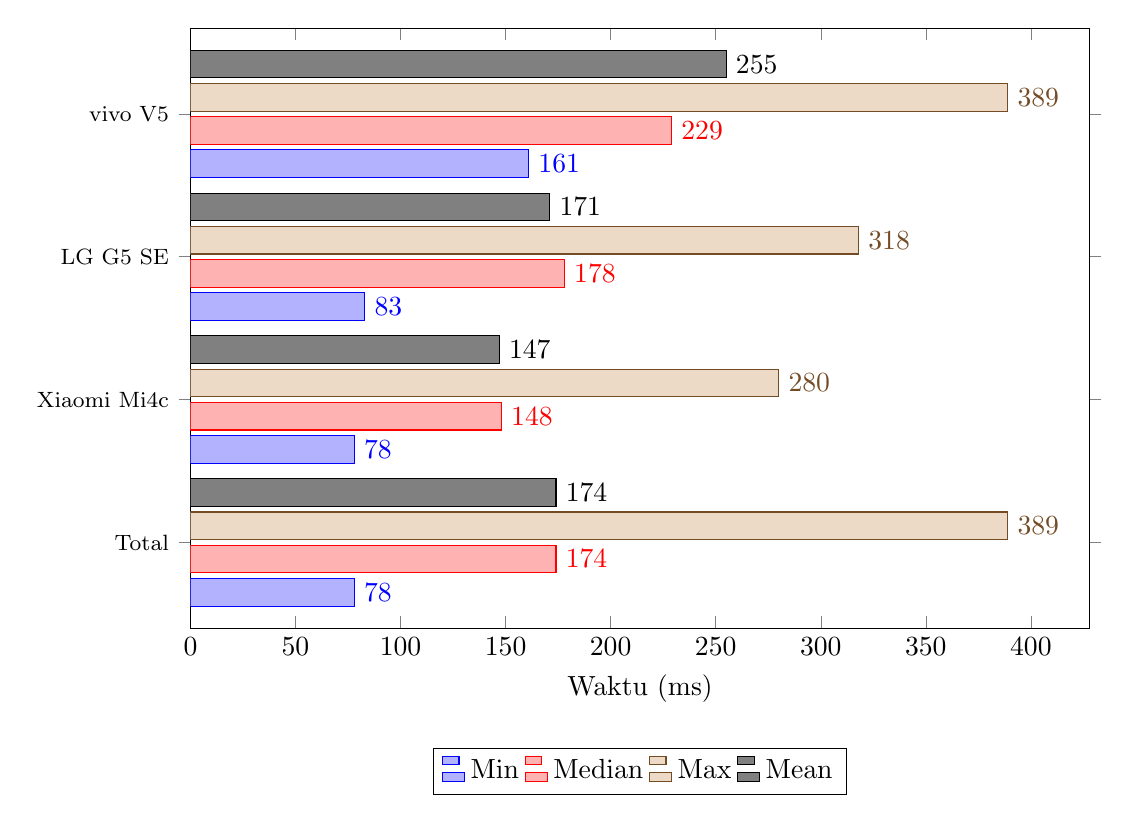
\begin{tikzpicture}
    \begin{axis}[
        xbar, xmin=0,
        y tick label style={font=\footnotesize},
        width=13cm, height=9.2cm, enlarge y limits=0.2,
        xlabel={Waktu (ms)},
        symbolic y coords={Total,Xiaomi Mi4c,LG G5 SE,vivo V5},
        ytick=data,
        nodes near coords, nodes near coords align={horizontal},
        legend style={at={(0.5,-0.20)},
        anchor=north,legend columns=-1},
        ]
        \addplot % Min
        coordinates 
        {(78,Total) (78,Xiaomi Mi4c) (83,LG G5 SE) (161,vivo V5)};
        
        \addplot % Median
        coordinates 
        {(174,Total) (148,Xiaomi Mi4c) (178,LG G5 SE) (229,vivo V5)};
        
        \addplot % Max
        coordinates 
        {(389,Total) (280,Xiaomi Mi4c) (318,LG G5 SE) (389,vivo V5)};

        \addplot % Mean
        coordinates
        {(174,Total) (147,Xiaomi Mi4c) (171,LG G5 SE) (255,vivo V5)};

        \legend{Min,Median,Max,Mean}
    \end{axis}
    \end{tikzpicture}
    \caption{Hasil pengujian kecepatan klasifikasi pada ponsel cerdas}
    \label{gambar:hasil-kecepatan}
\end{figure}

% Perlu dicatat bahwa kecepatan ini hanyalah pendekatan dari waktu komputasi yang sebenarnya. Waktu komputasi diukur dengan ponsel dalam keadaan seperti pada penggunaan sehari-hari, sehingga dipengaruhi oleh beberapa faktor lain seperti penjadwalan sistem operasi dan adanya aplikasi lain yang sedang berjalan di latar belakang.

\chapter{KESIMPULAN DAN SARAN}

\section{Kesimpulan}
Berdasarkan hasil pengujian yang telah dilakukan, kesimpulan yang dapat diambil adalah sebagai berikut:

\begin{enumerate}
    \item Telah berhasil dibuat sistem klasifikasi aktivitas manusia menggunakan \textit{Convolutional Neural Network} dan \textit{Long Short-Term Memory} untuk enam aktivitas sederhana, yaitu duduk, berjalan, berdiri, berlari, menaiki tangga dan menuruni tangga.
    \item Klasifikasi aktivitas manusia secara \textit{offline} pada data uji memperoleh akurasi 93,65\%, sedangkan klasifikasi \textit{online} pada ponsel cerdas dapat dilakukan dengan akurasi 89,757\%.
    \item Proses klasifikasi pada ponsel cerdas dapat dilakukan dengan rata-rata 174 ms, sehingga dinilai cukup baik untuk melakukan klasifikasi secara \textit{realtime}.
\end{enumerate}

\section{Saran}
Berikut beberapa saran untuk mengembangkan penelitian ini:

\begin{enumerate}
    \item Diperlukan penelitian lebih lanjut untuk mengenali aktivitas lainnya.
    \item Diperlukan penelitian lebih lanjut untuk meningkatkan akurasi klasifikasi, misalnya dengan menggunakan LSTM dua arah dan \textit{residual networks}.
    \item Diperlukan penelitian lebih lanjut untuk mengurangi \textit{overfitting} pada model.
\end{enumerate}



\bibliography{pustaka}

\end{document}
